% Adding a coloured vertical edge to the pages in the chapter
\ClearShipoutPicture
\AddToShipoutPicture{%
  \AtPageLowerLeft{%
    \checkoddpage
    \ifoddpage
      \begin{tikzpicture}[remember picture,overlay] % Odd page → right edge
        \draw[line width=80pt, colour_chapter6] 
             (\paperwidth,0) -- (\paperwidth,\paperheight);
      \end{tikzpicture}%
    \else
      \begin{tikzpicture}[remember picture,overlay] % Even page → left edge
        \draw[line width=80pt, colour_chapter6] 
             (0,0) -- (0,\paperheight);
      \end{tikzpicture}%
    \fi
  }%
}

%%%%%%%%%%%%%%%%%%%%%%%%%%%%%%%%%%%%%%%%%%%%%%%%%%%%%%%%%%%%%%%%%%%%
\chapter{Data-driven hydro-meteorological predictions of areas at risk of flash flood: from short- to medium-range lead times}
\label{data_driven_flash_floods_short_medium_range}
\graphicspath{{chapter_06/figures}{chapter_06/tables}}

\definecolor{colourTraining}{HTML}{800080}
\definecolor{colourOuterFolds}{HTML}{888888}
\definecolor{colourOuterTest}{HTML}{2CA58D}
\definecolor{colourInnerTraining}{HTML}{FF0066}
\definecolor{colourInnerValidation}{HTML}{E98A15}
\definecolor{colourTest}{HTML}{00B0F0}
%%%%%%%%%%%%%%%%%%%%%%%%%%%%%%%%%%%%%%%%%%%%%%%%%%%%%%%%%%%%%%%%%%%%

\underline{\textbf{Authors' contribution for this chapter:}} Fatima M. Pillosu designed the study, with advice from Mariana Clare, Florian Pappenberger, Hannah Cloke, and Christel Prudhomme, obtained the datasets, carried out the analysis, and led the writing of the manuscript. All authors assisted with writing the manuscript. Overall, 90\% of the writing was undertaken by Fatima M. Pillosu.

\vspace{\baselineskip}

\section*{PREFACE}
\addcontentsline{toc}{section}{PREFACE}

The second main analysis chapter (Chapter \ref{data_driven_flash_floods_short_medium_range}) develops a data-driven model that integrates multiple hydro-meteorological parameters to enhance the prediction capabilities of areas at risk of flash floods. Building upon the baseline established in Chapter \ref{flash_flood_focused_verification_rainfall_based_ff}, this investigation recognises that whilst rainfall magnitude, duration, and location constitute critical forcing mechanisms, flash flood occurrence emerges from complex interactions between meteorological inputs and catchment characteristics. The methodology incorporates antecedent soil moisture conditions, topographical features, and land cover properties to capture the nonlinear relationships governing flash flood generation, thereby transitioning from purely meteorological prediction towards a comprehensive hydro-meteorological framework. Furthermore, the chapter undertakes a systematic temporal analysis of forecast skill degradation across lead times extending to five days, establishing the practical boundaries within which operational decisions can be reliably supported. This temporal dimension proves essential for delineating the utility of forecasts across different emergency management phases—from immediate response activation at one-day lead times to strategic preparedness measures at extended horizons. Hence, in this chapter, \textcolor{colour_chapter6}{research question 2 (RQ2) "Is it feasible to develop data-driven predictions of areas at risk of flash flood at regional scale using reanalysis hydro-meteorological data and impact flash flood reports, and if so, up to what lead time?"} is answered. The second research component of this thesis is addressed here, i.e., the development of a proof-of-concept reanalysis-based and forecast-based - up to medium-range (day 5) - hydro-meteorological, data-driven predictions of areas at risk of flash floods.

\clearpage

\section*{ABSTRACT}
\addcontentsline{toc}{section}{ABSTRACT}

\clearpage



%%%%%%%%%%%%%%%%%%%%%%
\section{Introduction}
\label{data_driven_flash_floods_short_medium_range_introduction}


%%%%%%%%%%%%%%
\section{Data}
\label{data_driven_flash_floods_short_medium_range_data}
% To be completed.


%%%%%%%%%%%%%%%%%
\section{Methods}
\label{data_driven_flash_floods_short_medium_range_methods}

\subsection{Development of data-driven models}

\subsubsection{Model architecture selection}

Six distinct machine learning architectures were evaluated to identify the optimal approach for flash flood probability estimation: \textit{random forest} (with XGBoost and LightGBM implementations), \textit{gradient boosting} (with XGBoost, LightGBM, and CatBoost implementations), and a \textit{feed-forward neural network} (constructed using Keras and TensorFlow). These models were selected based on their proven efficacy in handling tabular data with class imbalance and their ability to capture complex non-linear relationships between hydro-meteorological predictors and flash flood occurrence \citep{Shwartz-Ziv_2022}.

Feed-forward \marginpara{Model architecture: feed-forward neural networks: TensorFlow and Keras implementation} neural networks represent the fundamental architecture of deep learning, comprising layers of interconnected nodes where information flows unidirectionally from input to output. Each neuron computes a weighted sum of its inputs, applies a non-linear activation function, and propagates the result forward. This architecture's universal approximation capability—the theoretical ability to approximate any continuous function given sufficient neurons—provides the flexibility to model complex non-linear relationships in hydro-meteorological applications. The multi-layer perceptron architecture employed in this study consists of fully connected layers with rectified linear unit (ReLU) activations, providing non-linearity whilst mitigating gradient vanishing issues. Dropout regularisation randomly deactivates neurons during training, creating an implicit ensemble effect that reduces overfitting. The back-propagation algorithm, combined with adaptive learning rate optimisation through Adam, enables efficient training even with limited positive examples in imbalanced datasets. The Keras implementation provides a high-level interface to TensorFlow's computational graph framework, enabling rapid prototyping whilst maintaining computational efficiency. The Sequential API facilitates straightforward construction of feed-forward architectures with customisable depth and width. The implementation leverages TensorFlow's automatic differentiation capabilities for gradient computation and supports various optimisation algorithms, loss functions, and regularisation techniques. For imbalanced classification, the class\_weight parameter in the fit method enables sample weighting to address class frequency disparities.

Gradient \marginpara{Model architecture: gradient boosting (XGBoost, LightGBM, and CatBoost implementations)} boosting represents a powerful ensemble technique that sequentially constructs decision trees, where each subsequent tree attempts to correct the residual errors of the preceding ensemble \citep{Bentéjac_2021}. The algorithm operates by fitting new models to the negative gradients of a differentiable loss function, effectively performing gradient descent in function space. This iterative refinement process enables the capture of complex non-linear relationships and interactions between features. The mathematical formulation frames boosting as an optimisation problem in function space, where the objective is to minimise the expected value of a loss function by iteratively adding weak learners. The use of shallow trees as base learners provides regularisation through structural constraints, whilst shrinkage parameters control the contribution of each tree to prevent overfitting. XGBoost (Extreme Gradient Boosting) enhances the traditional gradient boosting algorithm through several algorithmic innovations. The framework incorporates second-order Taylor expansion of the loss function, enabling more accurate optimisation steps. Regularisation terms in the objective function penalise model complexity through both L1 and L2 norms on leaf weights and the number of leaves. The column block structure for parallel processing, cache-aware access patterns, and out-of-core computation capabilities enable efficient training on large datasets. For imbalanced classification problems, XGBoost provides the \textit{scale\_pos\_weight} parameter to adjust for class frequencies directly in the loss function \citep{Chen_2016}. LightGBM (Light Gradient Boosting Machine) introduces novel techniques to accelerate training whilst maintaining accuracy. The Gradient-based One-Side Sampling (GOSS) retains instances with large gradients whilst randomly sampling from instances with small gradients, effectively focusing computational resources on difficult-to-classify examples. Exclusive Feature Bundling (EFB) reduces dimensionality by bundling mutually exclusive features, particularly beneficial for sparse datasets. The histogram-based algorithm and leaf-wise tree growth strategy enable faster convergence and better accuracy compared to level-wise approaches, though requiring careful regularisation to prevent overfitting \citep{Ke_2017}. CatBoost addresses several fundamental challenges in gradient boosting through innovative algorithmic solutions. The ordered boosting approach mitigates prediction shift—a subtle form of overfitting in gradient boosting—by using different data permutations for calculating gradients and applying models. This technique provides unbiased gradient estimates and improves generalisation. The algorithm's symmetric tree structure, whilst potentially less flexible than asymmetric trees, enables extremely fast inference and natural handling of categorical features through novel encoding schemes. For imbalanced datasets, CatBoost offers sophisticated class weighting mechanisms and custom loss functions optimised for rare event detection \citep{Prokhorenkova_2018}.

Random \marginpara{Model architecture: random forest (XGBoost and LightGBM implementations)} forest constitutes an ensemble learning method that constructs multiple decision trees during training and outputs predictions based on the mode of individual tree classifications for categorical targets or mean predictions for regression tasks \citep{Liu_2012}. The algorithm introduces randomness through two primary mechanisms: bootstrap aggregating (bagging), where each tree is trained on a random sample of the data with replacement, and random feature selection at each split, where only a subset of features is considered for determining the optimal partition. This dual randomisation strategy reduces overfitting and improves generalisation performance, particularly for high-dimensional datasets with complex feature interactions. The XGBoost implementation of random forest\footnote{https://xgboost.readthedocs.io/en/stable/tutorials/rf.html} adapts the gradient boosting framework to emulate a random forest behaviour by setting specific hyperparameters. This implementation maintains the core Random Forest principles whilst leveraging XGBoost's computational efficiency and regularisation capabilities. The key modifications include setting the number of parallel trees equal to the number of estimators, using a learning rate of 1.0, and disabling boosting rounds. This approach benefits from XGBoost's optimised handling of missing values, built-in cross-validation support, and efficient memory usage through its column block structure. The LightGBM implementation of random forest utilises gradient-based one-side sampling and exclusive feature bundling techniques, which significantly reduce computational complexity, whilst maintaining accuracy\footnote{https://lightgbm.readthedocs.io/en/latest/index.html}. The histogram-based algorithm constructs decision trees by bucketing continuous features into discrete bins, enabling faster split finding and reduced memory consumption. This implementation particularly excels with large-scale datasets and high-dimensional feature spaces.


\subsection{Feature engineering}

The data-driven models used primarily the raw variables as described in Section \ref{data_driven_flash_floods_short_medium_range_data}. The only variable engineered corresponds to the \textit{maximum probability of 24-hourly rainfall exceeding a specific threshold in adjacent grid-boxes}. This variable examines the probabilities in adjacent grid-boxes to that of interest, within an assigned radius, and selects the maximum value. This variable addresses two critical limitations that arise when the identification of areas at risk of flash floods relies solely on the probability of exceeding a certain threshold over the grid-box of interest. The first (meteorological) reason relates to the convective parametrisation scheme in global NWP models. In global NWP models, convective cells do not move, meaning the rainfall falls where the convective cell was generated by the model \citep{Doswell_2001}. In reality, convective cells move in the direction of the wind \citep{Doswell_2001}. A typical case corresponding to this scenario is a more or less organised convective system generated over a warm water body (e.g., the Mediterranean) that then moves onto land. Such a convective system, if conditions are favourable, may deliver significant rainfall amounts over land. However, as far as the model is concerned, the rainfall may fall over the water body, potentially causing a large underestimation of rainfall estimates over land. The second (hydrological) reason concerns the absence of water routing (over land or water courses) in this analysis. When rainfall occurs in one grid cell, it may flow downstream and cause flooding in adjacent cells. This routing effect becomes particularly important for fluvial flash floods in intermediate-sized catchments (100-500 km²), as seen, for example, during the severe flash floods occurred in Valencia in October 2024. Although ERA5's large grid cells (\sim31 km) may typically contain flash floods within their boundaries, downstream propagation can occur, with flash floods extending beyond the grid cell receiving rainfall and affecting neighbouring downstream grid-boxes.


\subsection{Repeated nested cross-validation for model training}

An important and long-standing concern in model training is \textit{overfitting} \citep{Ying_2019}. For predictive goals, overfitting degrades the generalisation of predictive performance to new data, and cross-validation is a technique that can help train models while limiting the risk of overfitting. 

Traditional \marginpara{Simple cross-validation to estimate model's generalisation capabilities} model training works by splitting the available data into a set of \textcolor{colourTraining}{\textit{training}} and \textcolor{colourTest}{\textit{test}} sets (Figure \ref{fig:cv_optuna}) where the model is fit to the training data and subsequently assessed based on its predictions to the test data \citep{Hastie_2009}. By repeating this process for \textit{k\_outer} number of splits (Figure \ref{fig:cv_optuna}, \textcolor{colourOuterFolds}{\textit{outer folds}}), the average predictive performance of one or more models can be estimated. The splits are created with the function \textit{RepeatedStratifiedKfold} in the SciKit-Learn Python. This function creates folds that preserve the original class distribution within each outer fold of the data partition\footnote{In standard k-fold cross-validation, data points are randomly assigned to folds without consideration of their class membership, which can result in significant variations in class proportions across folds, particularly problematic for imbalanced datasets. Stratified k-fold cross-validation addresses this limitation by ensuring that each fold maintains approximately the same percentage of samples from each class as the complete dataset.}, and repeats the partitioning n\_repeats times. 

Cross-validation \marginpara{Adoption of nested cross-validation to avoid data leakages when also tuning the model's hyperparameters} may also be used to estimate the model's hyperparameters. However, simple cross-validation uses the \textit{same data} for model selection and hyperparameter tuning, which may introduce \textit{data leakage}, thereby causing overfitting and compromising model generalisation capabilities \citep{Sasse_2025}. The magnitude of this effect depends on the dataset size, the balance between the frequency of binary events in the dataset, and the model's stability \citep{Sasse_2025}. A \textit{nested} cross-validation framework provides unbiased estimates of model performance when using severely imbalanced datasets, whilst simultaneously optimising hyperparameters. Each of the \textcolor{colourOuterFolds}{\textit{outer folds}} is divided into an \textcolor{colourOuterTest}{\textit{outer test fold}} and an outer training fold, which is split a \textit{k\_inner} number of times to create an \textcolor{colourInnerTraining}{\textit{inner training fold}} and an \textcolor{colourInnerValidation}{\textit{inner validation folds}}, preserving again the original class distribution within each inner fold (Figure \ref{fig:cv_optuna}). Hyperparameters are tuned over \textcolor{colourInnerTraining}{\textit{inner training folds}} and tested \textcolor{colourInnerValidation}{\textit{inner validation folds}}. When the hyperparameters are tuned, model generalisation is then tested over the \textcolor{colourOuterTest}{\textit{outer test folds}}.

\begin{figure}[htbp]
\centering
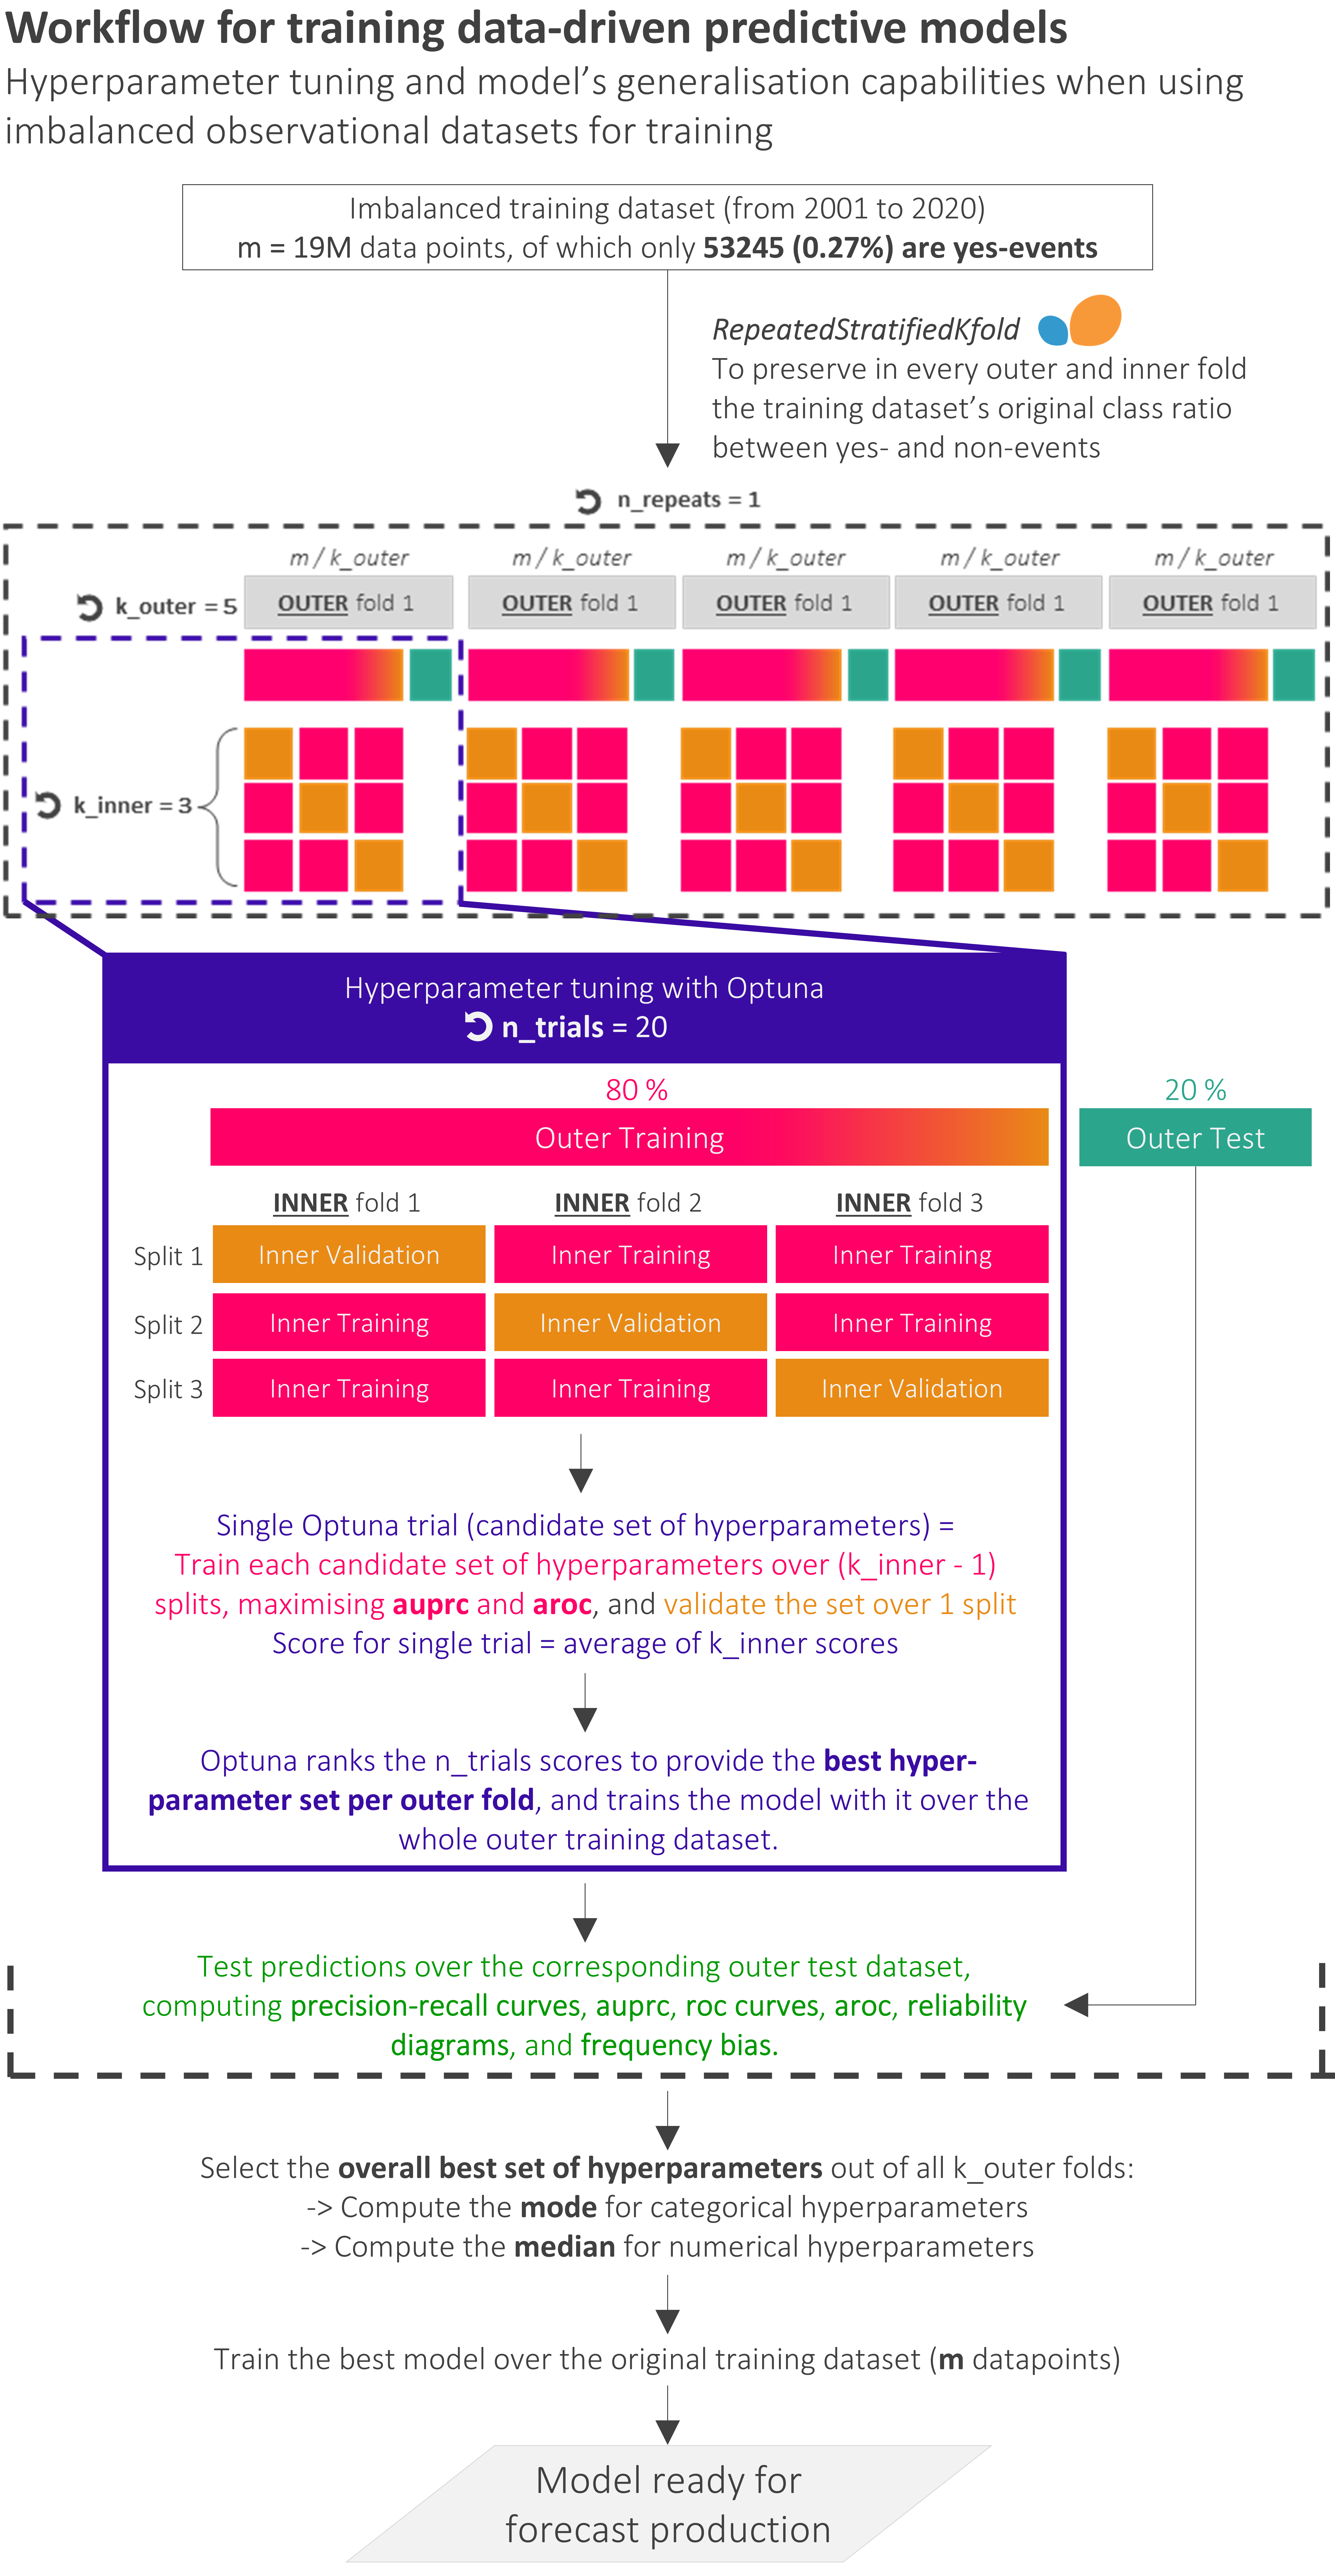
\includegraphics[scale = 0.9]{chapter_06/figures/cv_optuna.png}
\caption{\textbf{Workflow for the repeated nested cross-validation.} The outer cross-validation loop utilises Scikit-Learn's "RepeatedStratifiedKFold" function to create k\_outer = 5 outer folds (grey blocks) across n\_repeats = 1 iterations. Each \textcolor{colourOuterFolds}{\textit{outer fold}} maintains the class distribution of the \textcolor{colourTraining}{\textit{training dataset}}, and it is split into an outer training dataset (80\%, blocks in shades of pink and orange) and an \textcolor{colourOuterTest}{\textit{outer test dataset}} (20\%). Within each outer fold, a Bayesian hyperparameter tuning is performed employing the Optuna library through an inner cross-validation procedure over n\_trial = 20 repetitions. Each trial evaluates candidate hyperparameters by training on \textcolor{colourInnerTraining}{\textit{inner training folds}} and validating on \textcolor{colourInnerValidation}{\textit{inner validation folds}}, with performance measured as the mean AUC-ROC or AUC-PR. The optimal hyperparameter set, identified by maximising the selected evaluation metric, is used to train the final model on the complete outer training subset. Model performance is assessed on the held-out \textcolor{colourOuterTest}{\textit{outer test fold}} using AUC-ROC and AUC-PR. The best-performing fold is retrained on the original \textcolor{colourTraining}{\textit{training dataset}} for operational deployment. Independent, more extensive verification of the data-driven predictions is performed using the \textcolor{colourTest}{\textit{verification dataset}}, considering the Precision-Recall curve and AUC-PR, the ROC curve and AUC-ROC, reliability diagrams, and frequency bias.}
\label{fig:cv_optuna}
\end{figure}


\subsection{Hyperparameter tuning}

The \marginpara{Hyperparameter tuning: Optuna implementation} hyperparameter tuning was conducted using the Python library Optuna \citep{Akiba_2019}. The framework implements a Bayesian optimisation algorithm, primarily utilising the Tree-structured Parzen Estimator (TPE) sampler, which models the relationship between hyperparameters and objective function values to navigate high-dimensional search spaces efficiently. This approach significantly outperforms traditional grid search and random search methods, particularly when computational resources are limited or when the hyperparameter space is complex and continuous. The framework's architecture enables dynamic construction of search spaces where hyperparameters can be conditionally dependent on one another. Optuna's pruning capabilities represent a crucial innovation for computationally intensive tasks, allowing early termination of unpromising trials based on intermediate performance metrics. Moreover, the MedianPruner implementations monitor trial progress and eliminate configurations that are statistically unlikely to surpass previously observed performance, thereby focusing computational resources on promising regions of the hyperparameter space. This feature proves particularly valuable when training deep neural networks or large ensemble models, where individual trial evaluation may require substantial time. Optuna's integration with popular machine learning frameworks such as XGBoost, LightGBM, CatBoost, and TensorFlow handle framework-specific optimisations such as early stopping criteria and validation monitoring, whilst maintaining compatibility with Optuna's pruning mechanisms. Finally, the comprehensive logging and visualisation capabilities facilitate post-hoc analysis of optimisation trajectories, parameter importance assessment, and convergence diagnostics, providing valuable insights into model behaviour and hyperparameter interactions.

The Bayesian optimisation process conducted through Optuna evaluated n\_trial = 20 distinct hyperparameter configurations, with each trial exploring different regions of the search space guided by the Tree-structured Parzen Estimator algorithm.


\subsection{Loss functions}

The training framework implements a dual-strategy approach to address class imbalance through loss function configuration, enabling empirical determination of whether class weighting improves predictive performance for the specific characteristics of flash flood data. 

For \marginpara{Standard loss functions for balanced datasets} balanced datasets or when class imbalance is not a primary concern, the standard \textit{binary cross-entropy (BCE) loss function} is employed without modification. The standard BCE treats the binary classes equally, computing the negative log-likelihood of the predicted probabilities without any weighting mechanism. For tree-based models, the equivalent implementations include \textit{binary:logistic} objective for XGBoost, \textit{binary} objective for LightGBM, and \textit{Logloss} objective for CatBoost. These standard formulations assume that misclassification costs are symmetric between classes and that the training data adequately represents the true class distribution, making them suitable when positive and negative instances occur with comparable frequency.

Due \marginpara{Specialised loss functions for imbalanced datasets} to the severe class imbalance inherent in the problem considered in this thesis, the \textit{weighted binary cross-entropy (W-BCE) loss function} is also considered. It assigns differential importance to minority class instances through an optimisable positive class weight parameter (i.e., the class weights are themselves a hyperparameter optimised with Optuna), within the range [1.0, 10.0]. This weighting mechanism compensates for the scarcity of positive examples by increasing their contribution to the overall loss calculation, thereby preventing the model from converging to a trivial solution that simply predicts the majority class, i.e., it penalises misclassifications of rare flash flood events more heavily than false positives. The implementation manifests differently across frameworks: XGBoost and LightGBM utilise the \textit{scale\_pos\_weight} parameter to directly multiply the loss contribution of positive instances, whilst CatBoost employs the \textit{CrossEntropy loss function} with inherent class weighting capabilities. For neural networks, the Keras implementation applies \textit{class weights during batch gradient computation}, effectively rebalancing the optimisation landscape to ensure adequate representation of rare events.


\subsection{Verification scores}
\label{data_driven_flash_floods_short_medium_range_methods_verif_scores}
%To be completed. Similar to that one in Chapter 5. 



%%%%%%%%%%%%%%%%%
\section{Results}
\label{data_driven_flash_floods_short_medium_range_results}

\subsection{Model training}

The \marginpara{Model's hyperparameter optimisation} hyperparameter optimisation history plot (Figure \ref{fig:optuna_history}) shows the overall good performance of the Optuna library in identifying quickly (within the first 10 trial, orange lines) and with relatively small variations (grey lines) the sets of hyperparameters that maximise the chosen evaluation metrics (AUC-ROC and AUC-PR). Performance remains fairly consistent between different outer folds (lines in shades of grey and orange). The optimisation histories for AUC-ROC (Figure \ref{fig:optuna_history}a-l) and AUC-PR (Figure \ref{fig:optuna_history}m-x) are very similar, with plots for loss functions specific for imbalanced datasets (Figure \ref{fig:optuna_history}g-l and s-x) showing more variability, but in general better overall performance, than those for more general loss functions (Figure \ref{fig:optuna_history}a-f and m-r). 

\begin{figure}[htbp]
\centering
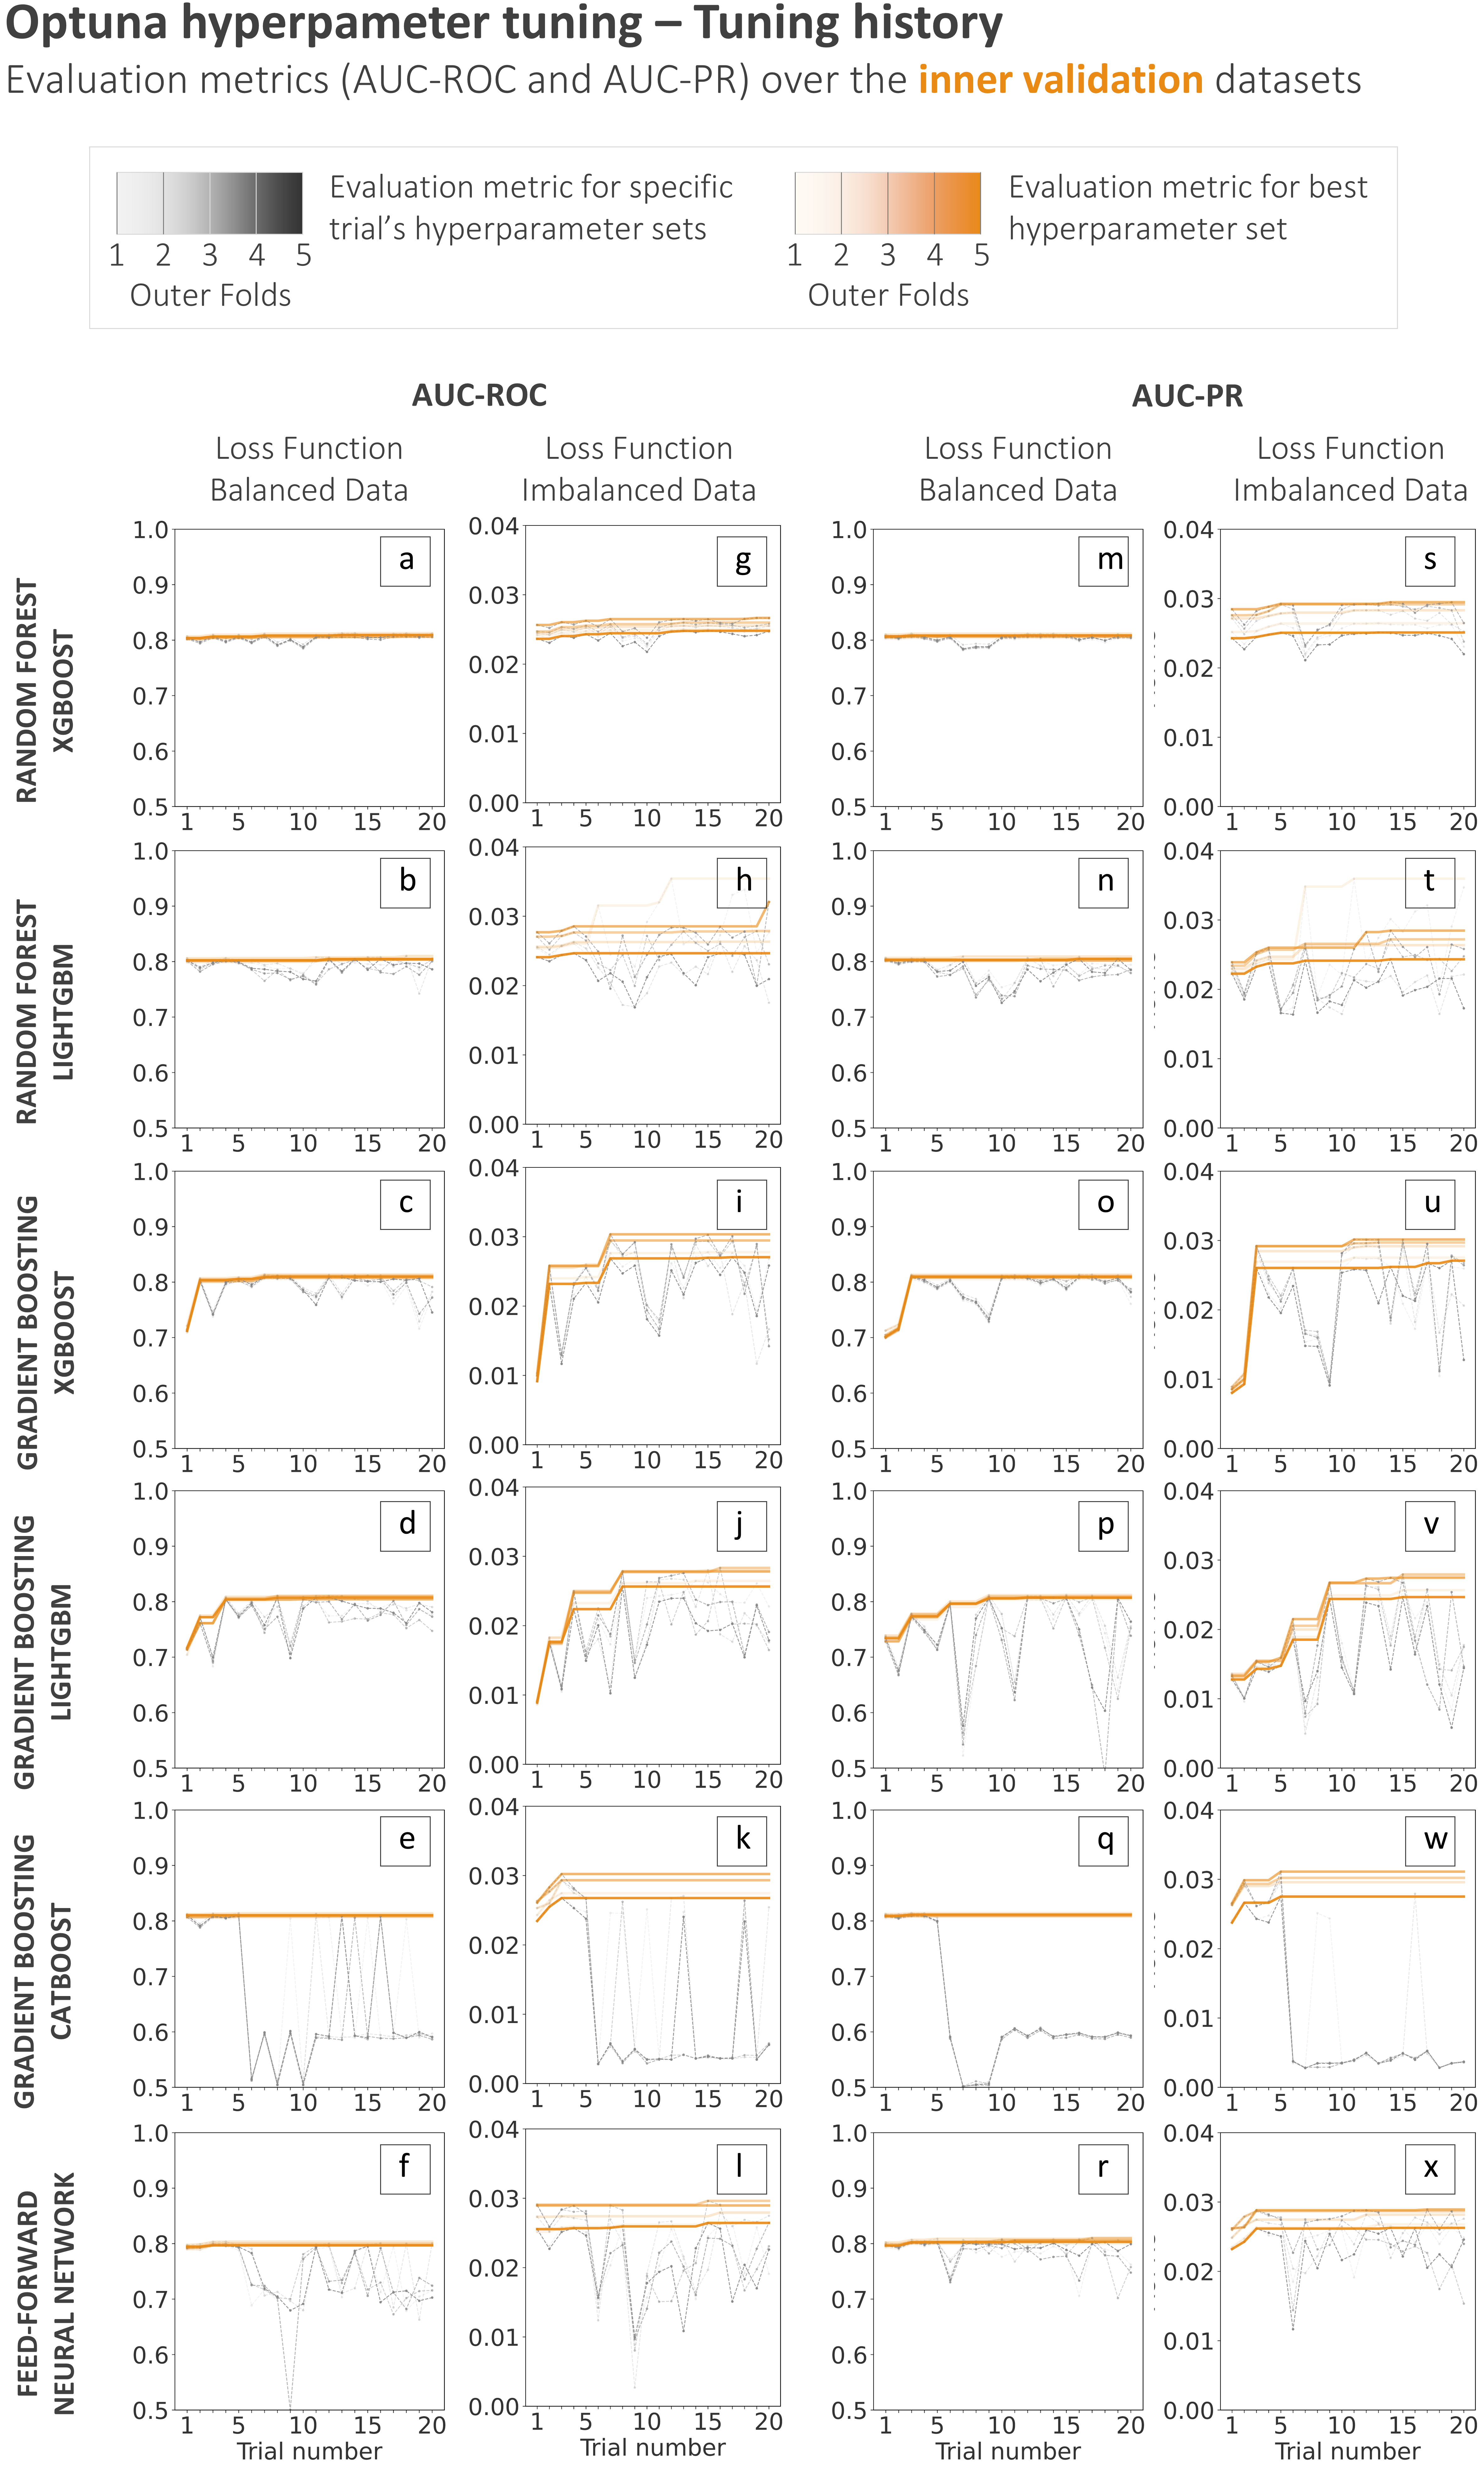
\includegraphics[scale=0.85]{optuna_history.png}
\caption{\textbf{Optuna's hyperparameter optimisation history.} Evolution of the two evaluation metrics (AUC-ROC, panels (a) to (l) - and AUC-PR, panels (m) to (x)) maximised during the 20 trials run over the \textcolor{colourInnerValidation}{\textit{inner validation folds}} to tune the hyperparameters of six data-driven models (from top to bottom): random forest XGBoost, random forest LightGBM, gradient boosting XGBoost, gradient boosting LightGBM, gradient boosting CatBoost, and feed-forward neural network. The lines in shades of grey indicate individual trial performances, whilst lines in shades of orange highlight the best-performing hyperparameter set, identified by Optuna's Bayesian optimisation process. The shades of grey and orange represent the values of the evaluation metrics for each outer fold (lightest shade for the first outer fold and darkest for the latest). Panels (a) to (f) and (m) to (r) represents the results obtained using the standard binary cross-entropy loss functions - mostly used for balanced datasets - whilst panels (g) to (l) and (s) to (x) present the outcomes obtained with the weighted loss functions (specifically configured for imbalanced data).}
\label{fig:optuna_history}
\end{figure}

The \marginpara{Optuna's training times} training times reveal substantial computational differences across model architectures (Figure \ref{fig:optuna_training_time}). Decision-tree-based implementations (except for CatBoost) demonstrate more efficient training times. On average, the training time per outer fold remains between 75 and 100 seconds, with peaks that do not exceed 500 seconds. CatBoost's training times are around 500 seconds per outer fold, with peaks reaching 2000 seconds. The feed-forward neural network exhibits the longest training times among all models, with an average training time of around 2000 seconds and peaks ranging from 4000 to 6000 seconds. These times indicate that it requires \sim20 minutes per outer fold to optimise hyperparameters and train the decision-tree-based models (except for CatBoost), compared to \sim2.5 and \sim8 hours per outer fold, respectively, for CatBoost and the feed-forward neural network. The choice of loss function and evaluation metric shows minimal impact on training duration across all architectures.

\begin{figure}[htbp]
\centering
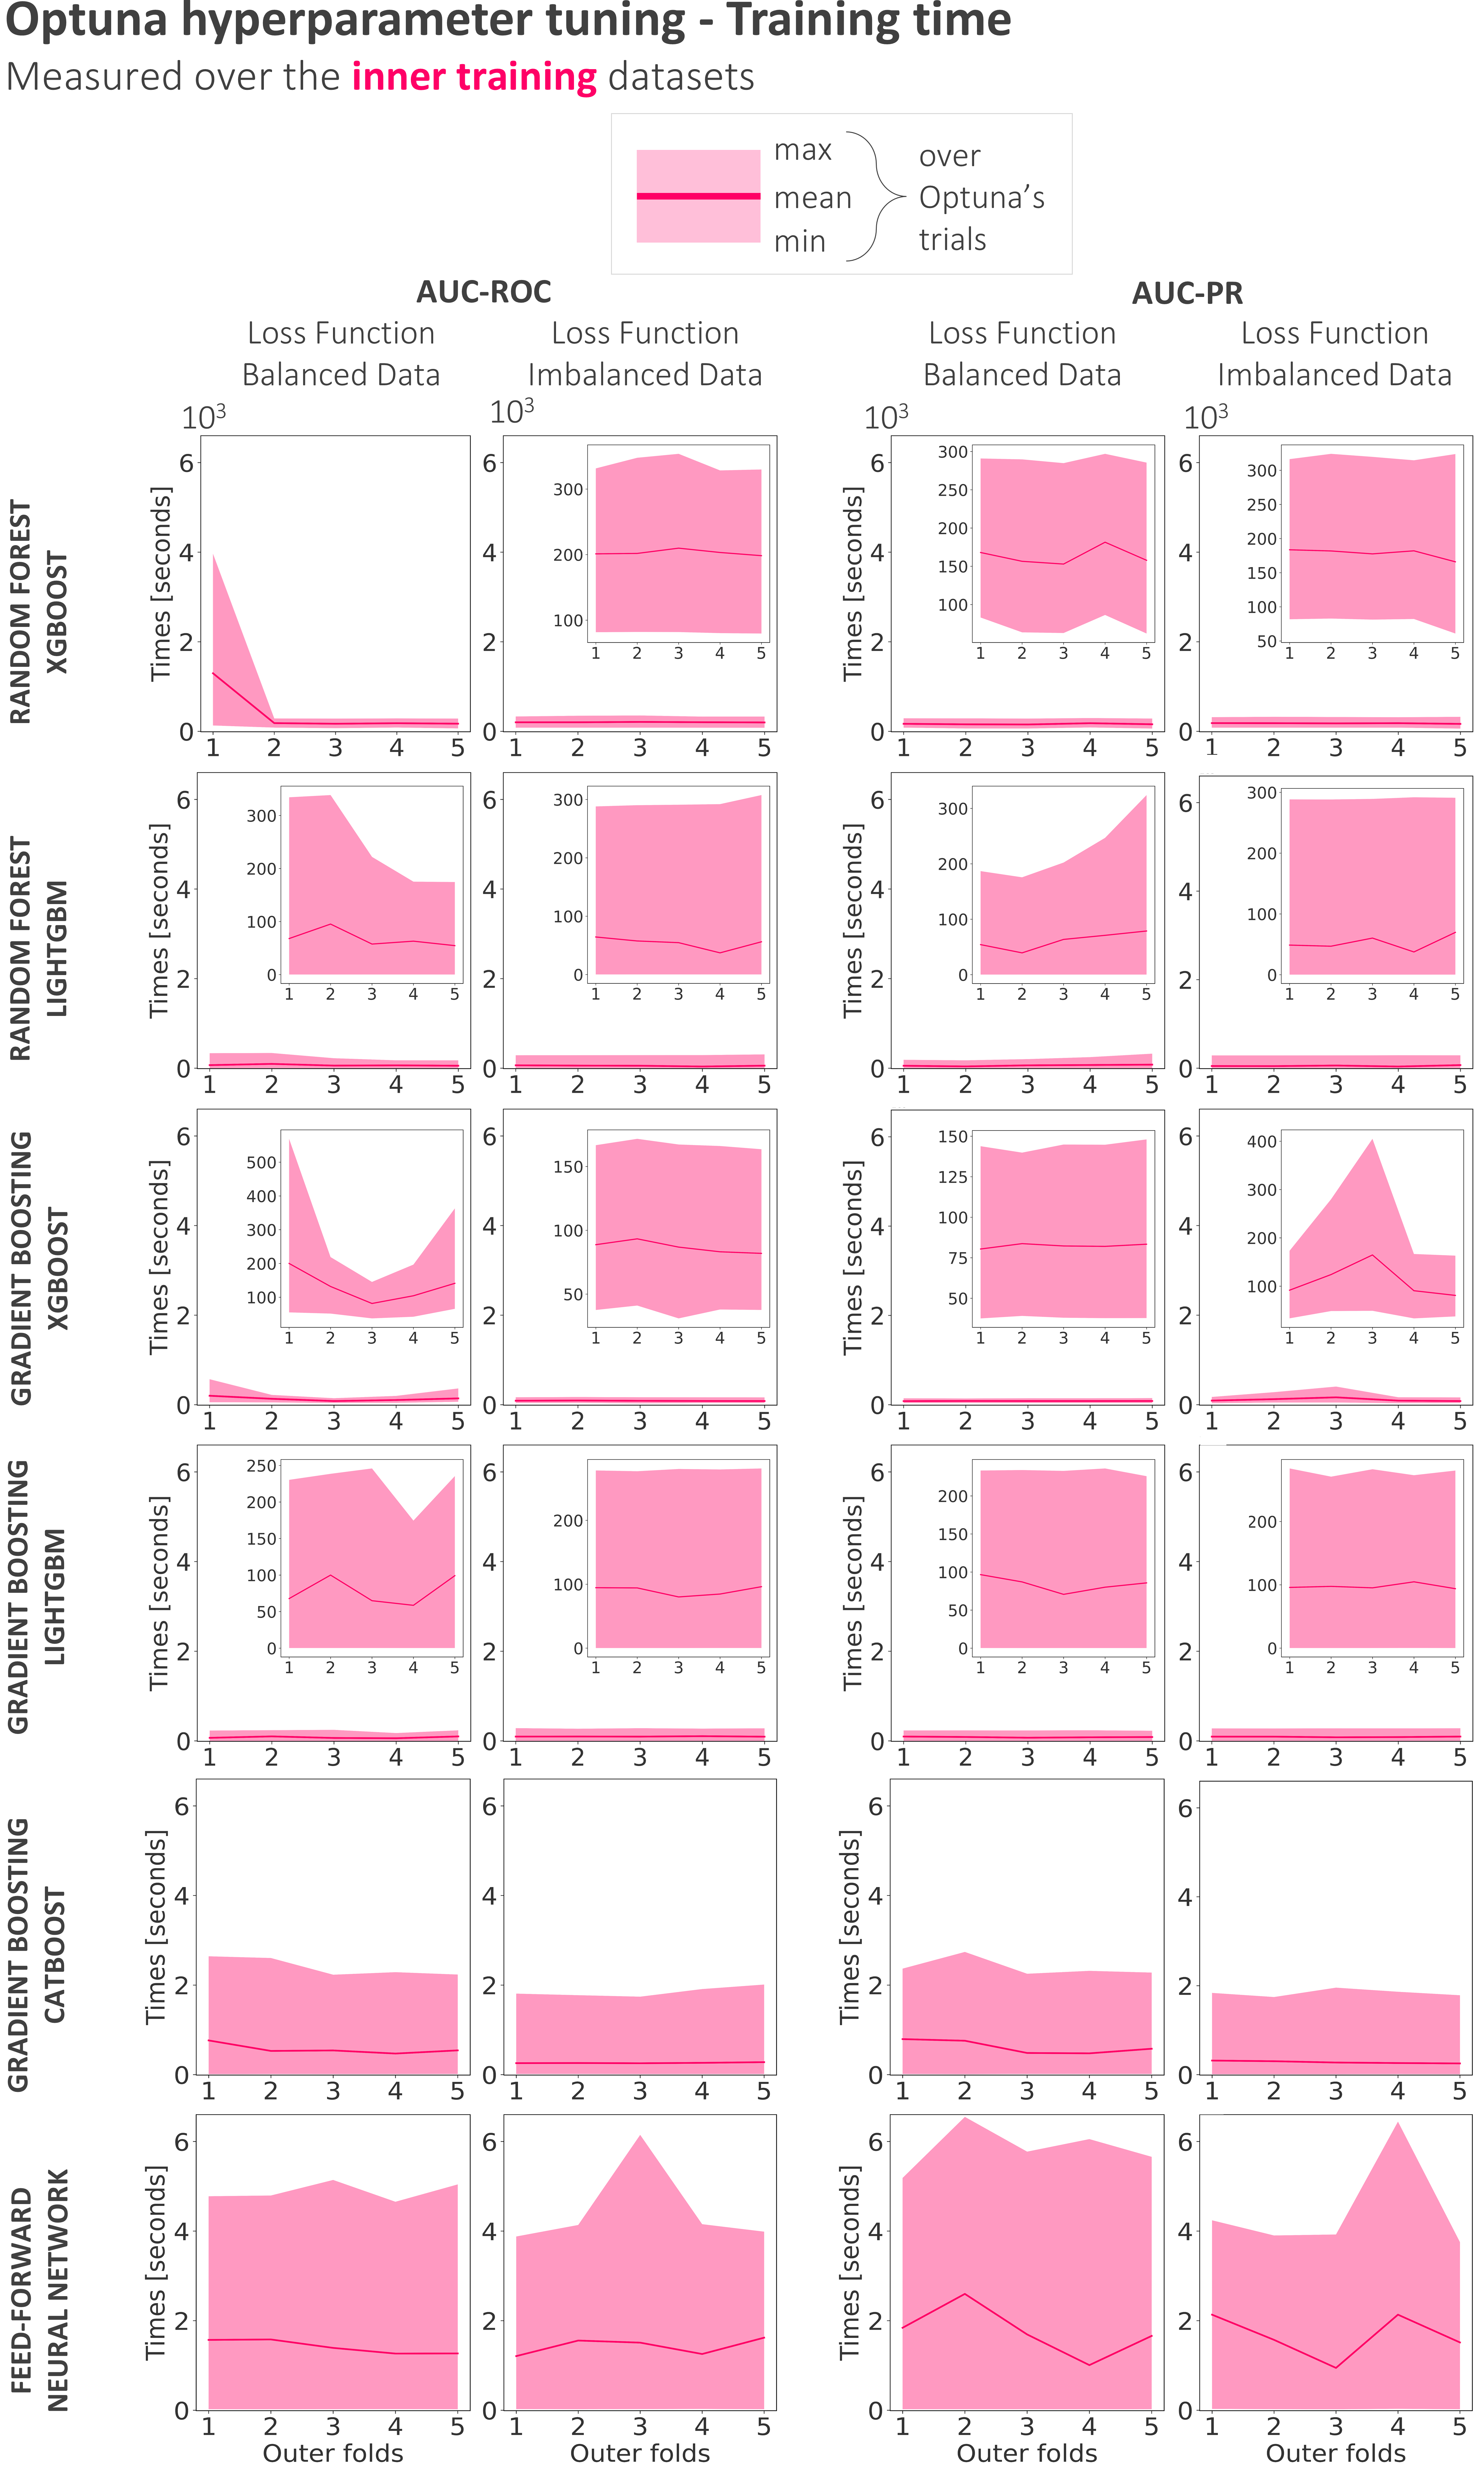
\includegraphics[scale=0.85]{optuna_time_training.png}
\caption{\textbf{Optuna's training time.} Evolution of training times (in seconds) for each k\_outer=5 outer folds across the n\_trials = 20 trials run over the \textcolor{colourInnerTraining}{\textit{inner training folds}} (the solid line represents the mean while the shaded area represents the minimum and maximum values). The training times for six data-driven models (from top to bottom) are shown: random forest XGBoost, random forest LightGBM, gradient boosting XGBoost, gradient boosting LightGBM, gradient boosting CatBoost, and feed-forward neural network. Training times are shown for both evaluation metrics (AUC-ROC - panels (a) to (l) - and AUC-PR - panels (m) to (x)) and loss function configurations (balanced and imbalanced datasets). Inset plots provide magnified views where appropriate.}
\label{fig:optuna_time_training}
\end{figure}

The \marginpara{Nested cross-validation: model generalisation} close values for both evaluation metrics (AUC-ROC and AUC-PR) estimated over the \textcolor{colourInnerValidation}{\textit{inner validation folds}} and the \textcolor{colourOuterTest}{\textit{outer test folds}} show the robustness of the nested cross-validation framework in mitigating overfitting during hyperparameter optimisation  (Figure \ref{fig:optuna_evaluation_metrics}). The fact that outer test performance remains generally bounded or close to the performance ranges estimated over the inner validation folds demonstrates that Optuna's Bayesian optimisation successfully identified hyperparameter configurations with robust generalisation capabilities to previously unseen data. The comparative analysis reveals minimal divergence between models trained with standard binary cross-entropy and those employing weighted loss functions (formulated specifically for class-imbalanced datasets). This observation holds for both evaluation metrics. Across the evaluated models, performance metrics demonstrate remarkable consistency, with the notable exception of CatBoost. Specifically, mean AUC-ROC values cluster between 0.7 and 0.8, whilst CatBoost exhibits inferior performance with values between 0.6 and 0.7. Similarly, mean AUC-PR values range from 0.02 to 0.03 across most models, with CatBoost again demonstrating diminished performance with values between 0.01 and 0.02. For both metrics, random forest implementations exhibit the narrowest bands, followed by gradient boosting implementations (except for CatBoost, which displays the widest bands among all models) and the feed-forward neural network. The wider bands for CatBoost exhibit greater sensitivity to hyperparameter choices and require more careful tuning to achieve optimal results. Random forest implementations exhibit the most constrained performance bands, indicating robust hyperparameter spaces that yield consistent results across outer folds. Gradient boosting implementations (except for CatBoost) and the feed-forward neural network demonstrate intermediate variability. CatBoost exhibits the broadest performance bands amongst all evaluated models, suggesting that CatBoost's hyperparameter space possesses heightened sensitivity, necessitating more meticulous optimisation procedures to achieve competitive performance levels.

\begin{figure}[htbp]
\centering
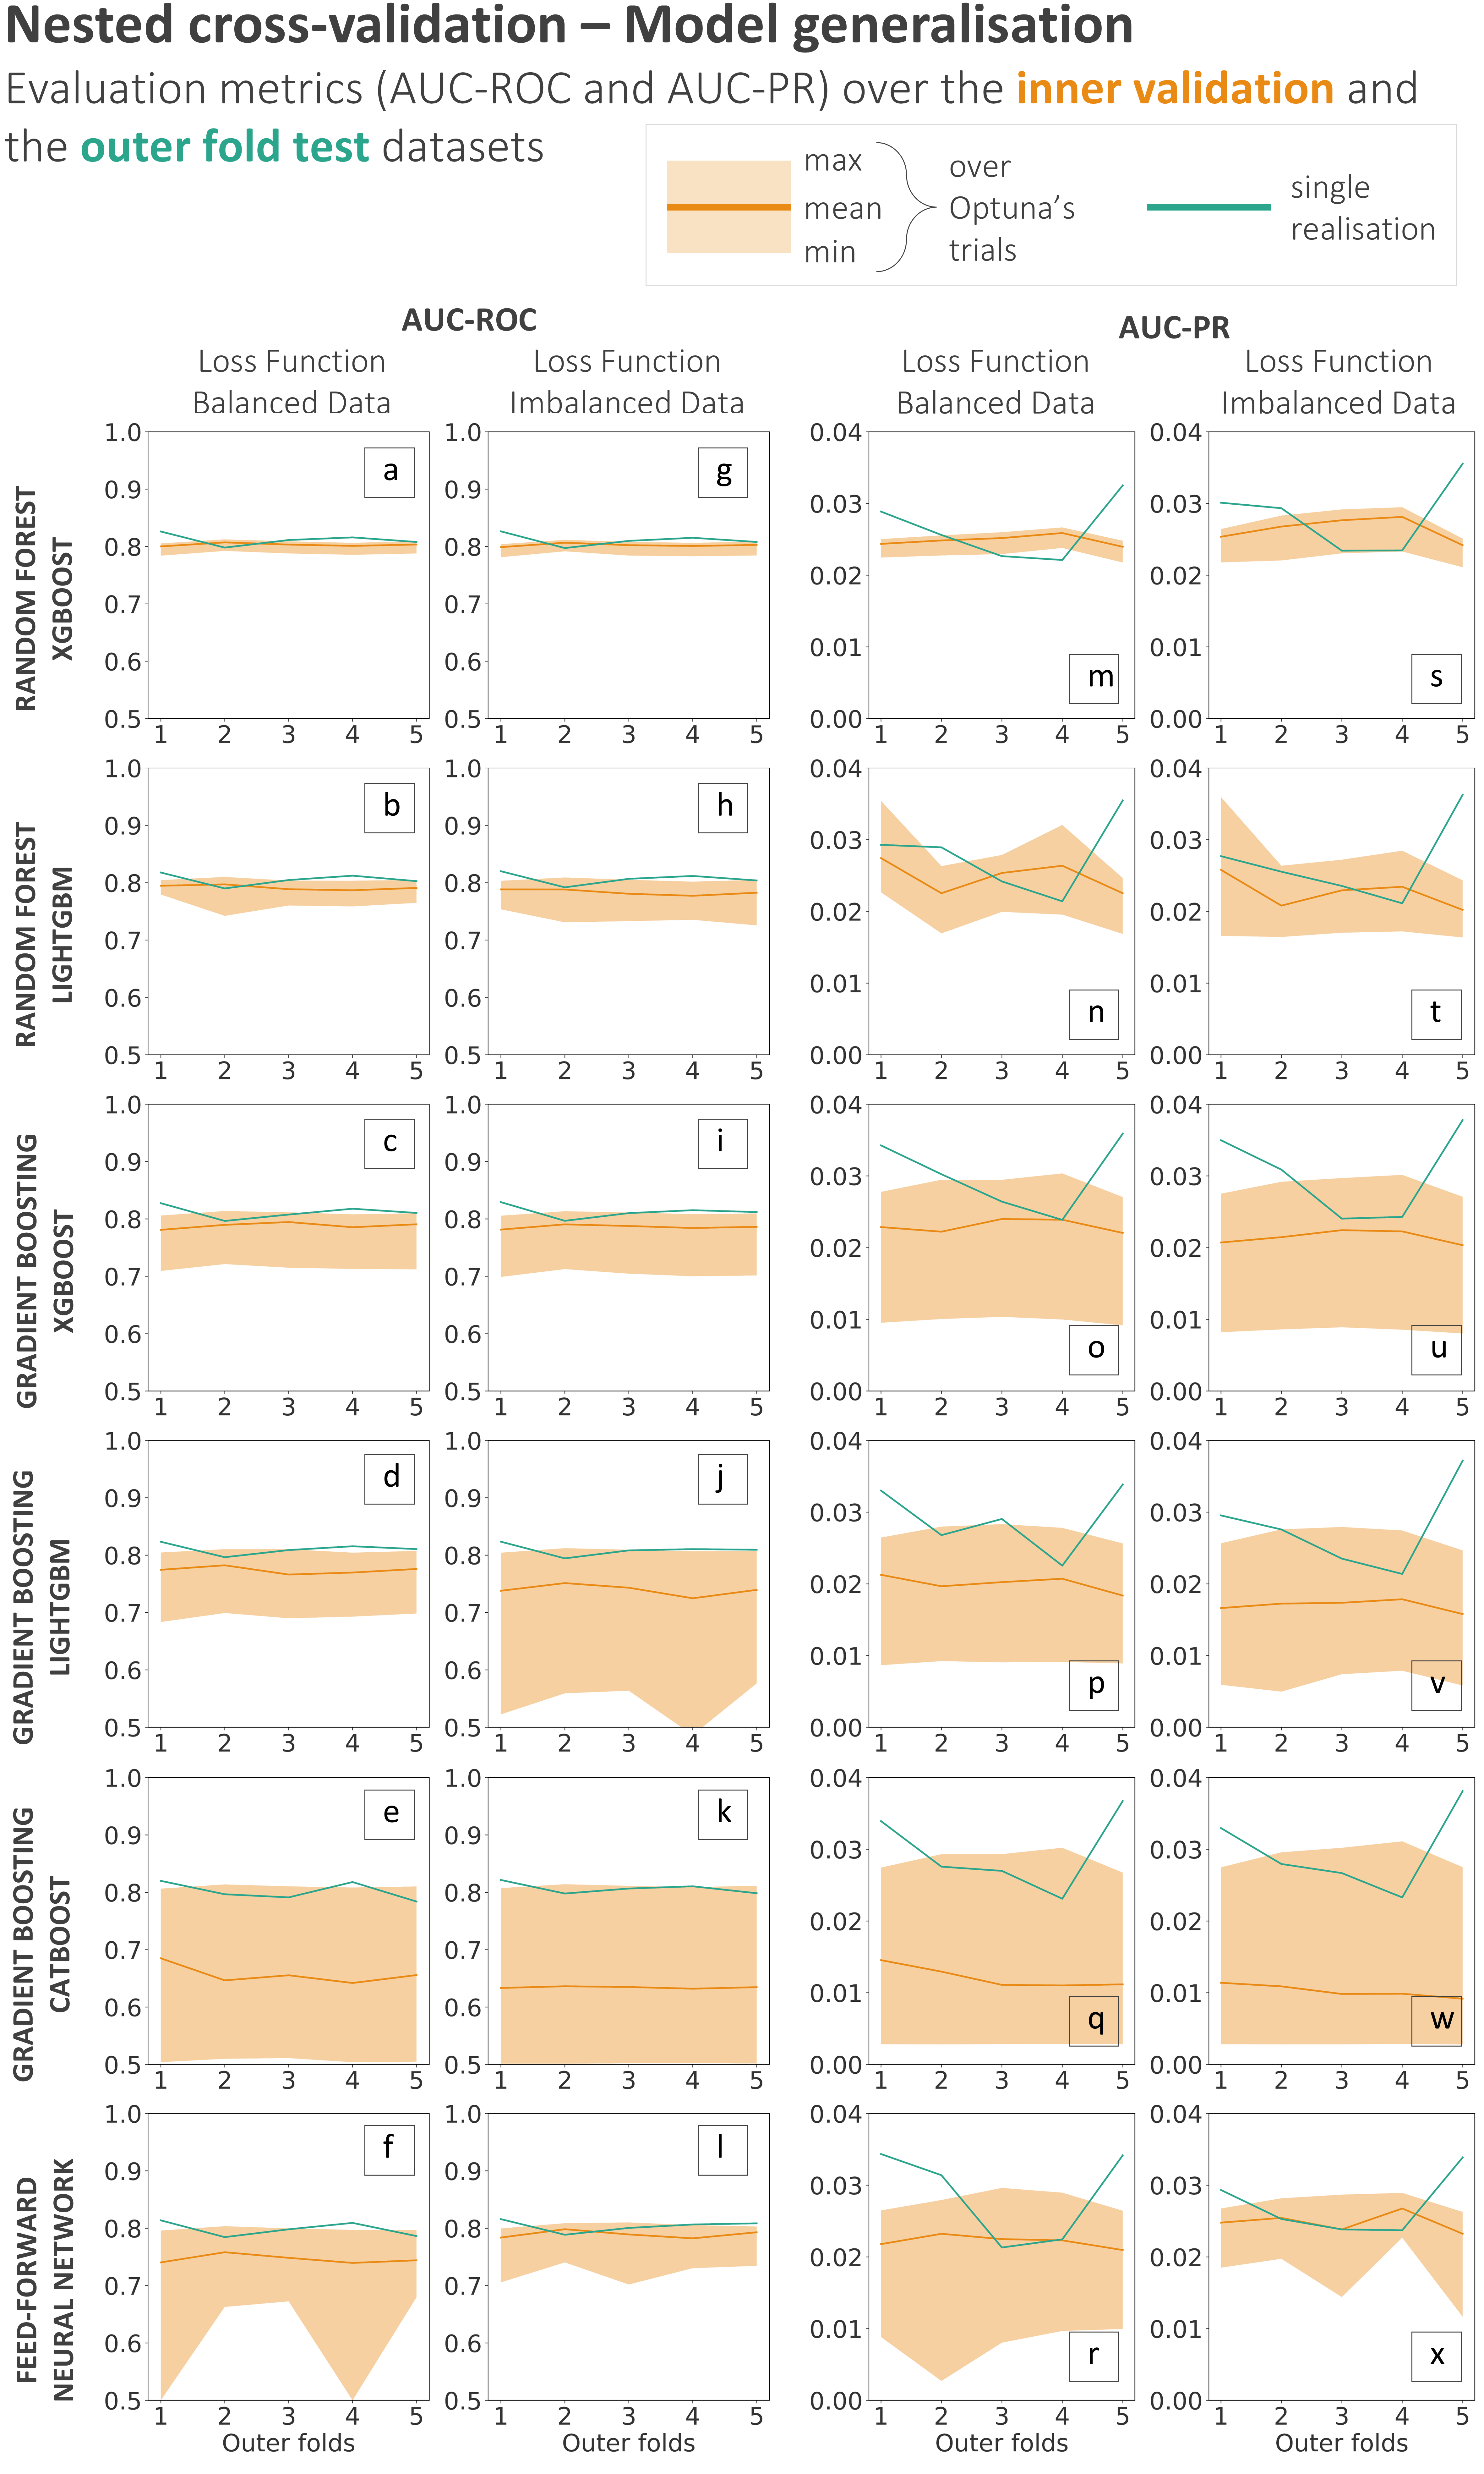
\includegraphics[scale=0.9]{chapter_06/figures/optuna_evaluation_metrics.png}
\caption{\textbf{Model generalisation from nested cross-validation} Values of the two evaluation metrics (AUC-ROC, panels (a) to (l) - and AUC-PR, panels (m) to (x)) across the 20 trials run over the \textcolor{colourInnerValidation}{\textit{inner validation folds}} (the \textcolor{colourInnerValidation}{solid line} represents the mean while the \textcolor{colourInnerValidation}{shaded area} represents the minimum and maximum values) and the \textcolor{colourOuterTest}{\textit{outer test fold}} (the \textcolor{colourOuterTest}{solid line} correspond to the single realisation per outer fold). Panels (a) to (f) and (m) to (r) represents the results obtained using the standard binary cross-entropy loss functions - mostly used for balanced datasets - whilst panels (g) to (l) and (s) to (x) present the outcomes obtained with the weighted loss functions (specifically configured for imbalanced data).}
\label{fig:optuna_evaluation_metrics}
\end{figure}


\subsubsection{Hyperparameter importance}

The \marginpara{Hyperparameter importance: gradient boosting implementations} hyperparameter importance analysis for XGBoost and LightGBM gradient boosting implementations reveals that maximum depth and learning rate consistently emerge as the most influential parameters. This aspect suggests that optimal performance depends fundamentally on striking a balance between model complexity and convergence dynamics. Maximum depth controls the model's capacity to capture complex hydro-meteorological interactions, whilst learning rate determines the magnitude of iterative corrections, requiring careful calibration to preserve gradient signals from rare positive events. LightGBM demonstrates additional sensitivity to the number of estimators due to its leaf-wise tree construction, producing more informative individual trees that necessitate precise ensemble size optimisation. In contrast, XGBoost's level-wise approach generates simpler trees that plateau predictably, reducing the criticality of this parameter. Notably, the positive class weight parameter exhibits a generally lower influence across both implementations, suggesting that structural parameters governing tree complexity and learning dynamics exert a greater impact on minority class detection than explicit re-weighting strategies. Thus, this emphasises the primacy of architectural optimisation over class balancing approaches. CatBoost exhibits considerable variability in the hyperparameters that most strongly influence model performance, with this variability dependent on both the chosen evaluation metric and the loss function configuration. When optimising for AUC-ROC, a set of parameters proves critical (e.g. depth and learning rate), yet these same parameters have minimal impact when considering AUC-PR. Furthermore, the implementation of weighted loss functions fundamentally alters the previously seen importance rankings, creating distinct optimisation priorities for balanced versus imbalanced scenarios. Unlike XGBoost and LightGBM, where maximum depth and learning rate consistently dominate, CatBoost lacks such universal governing parameters. The absence of consistent parameter hierarchies suggests that CatBoost's distinctive algorithmic approach generates a more complex hyperparameter space. 

\begin{figure}[htbp]
\centering
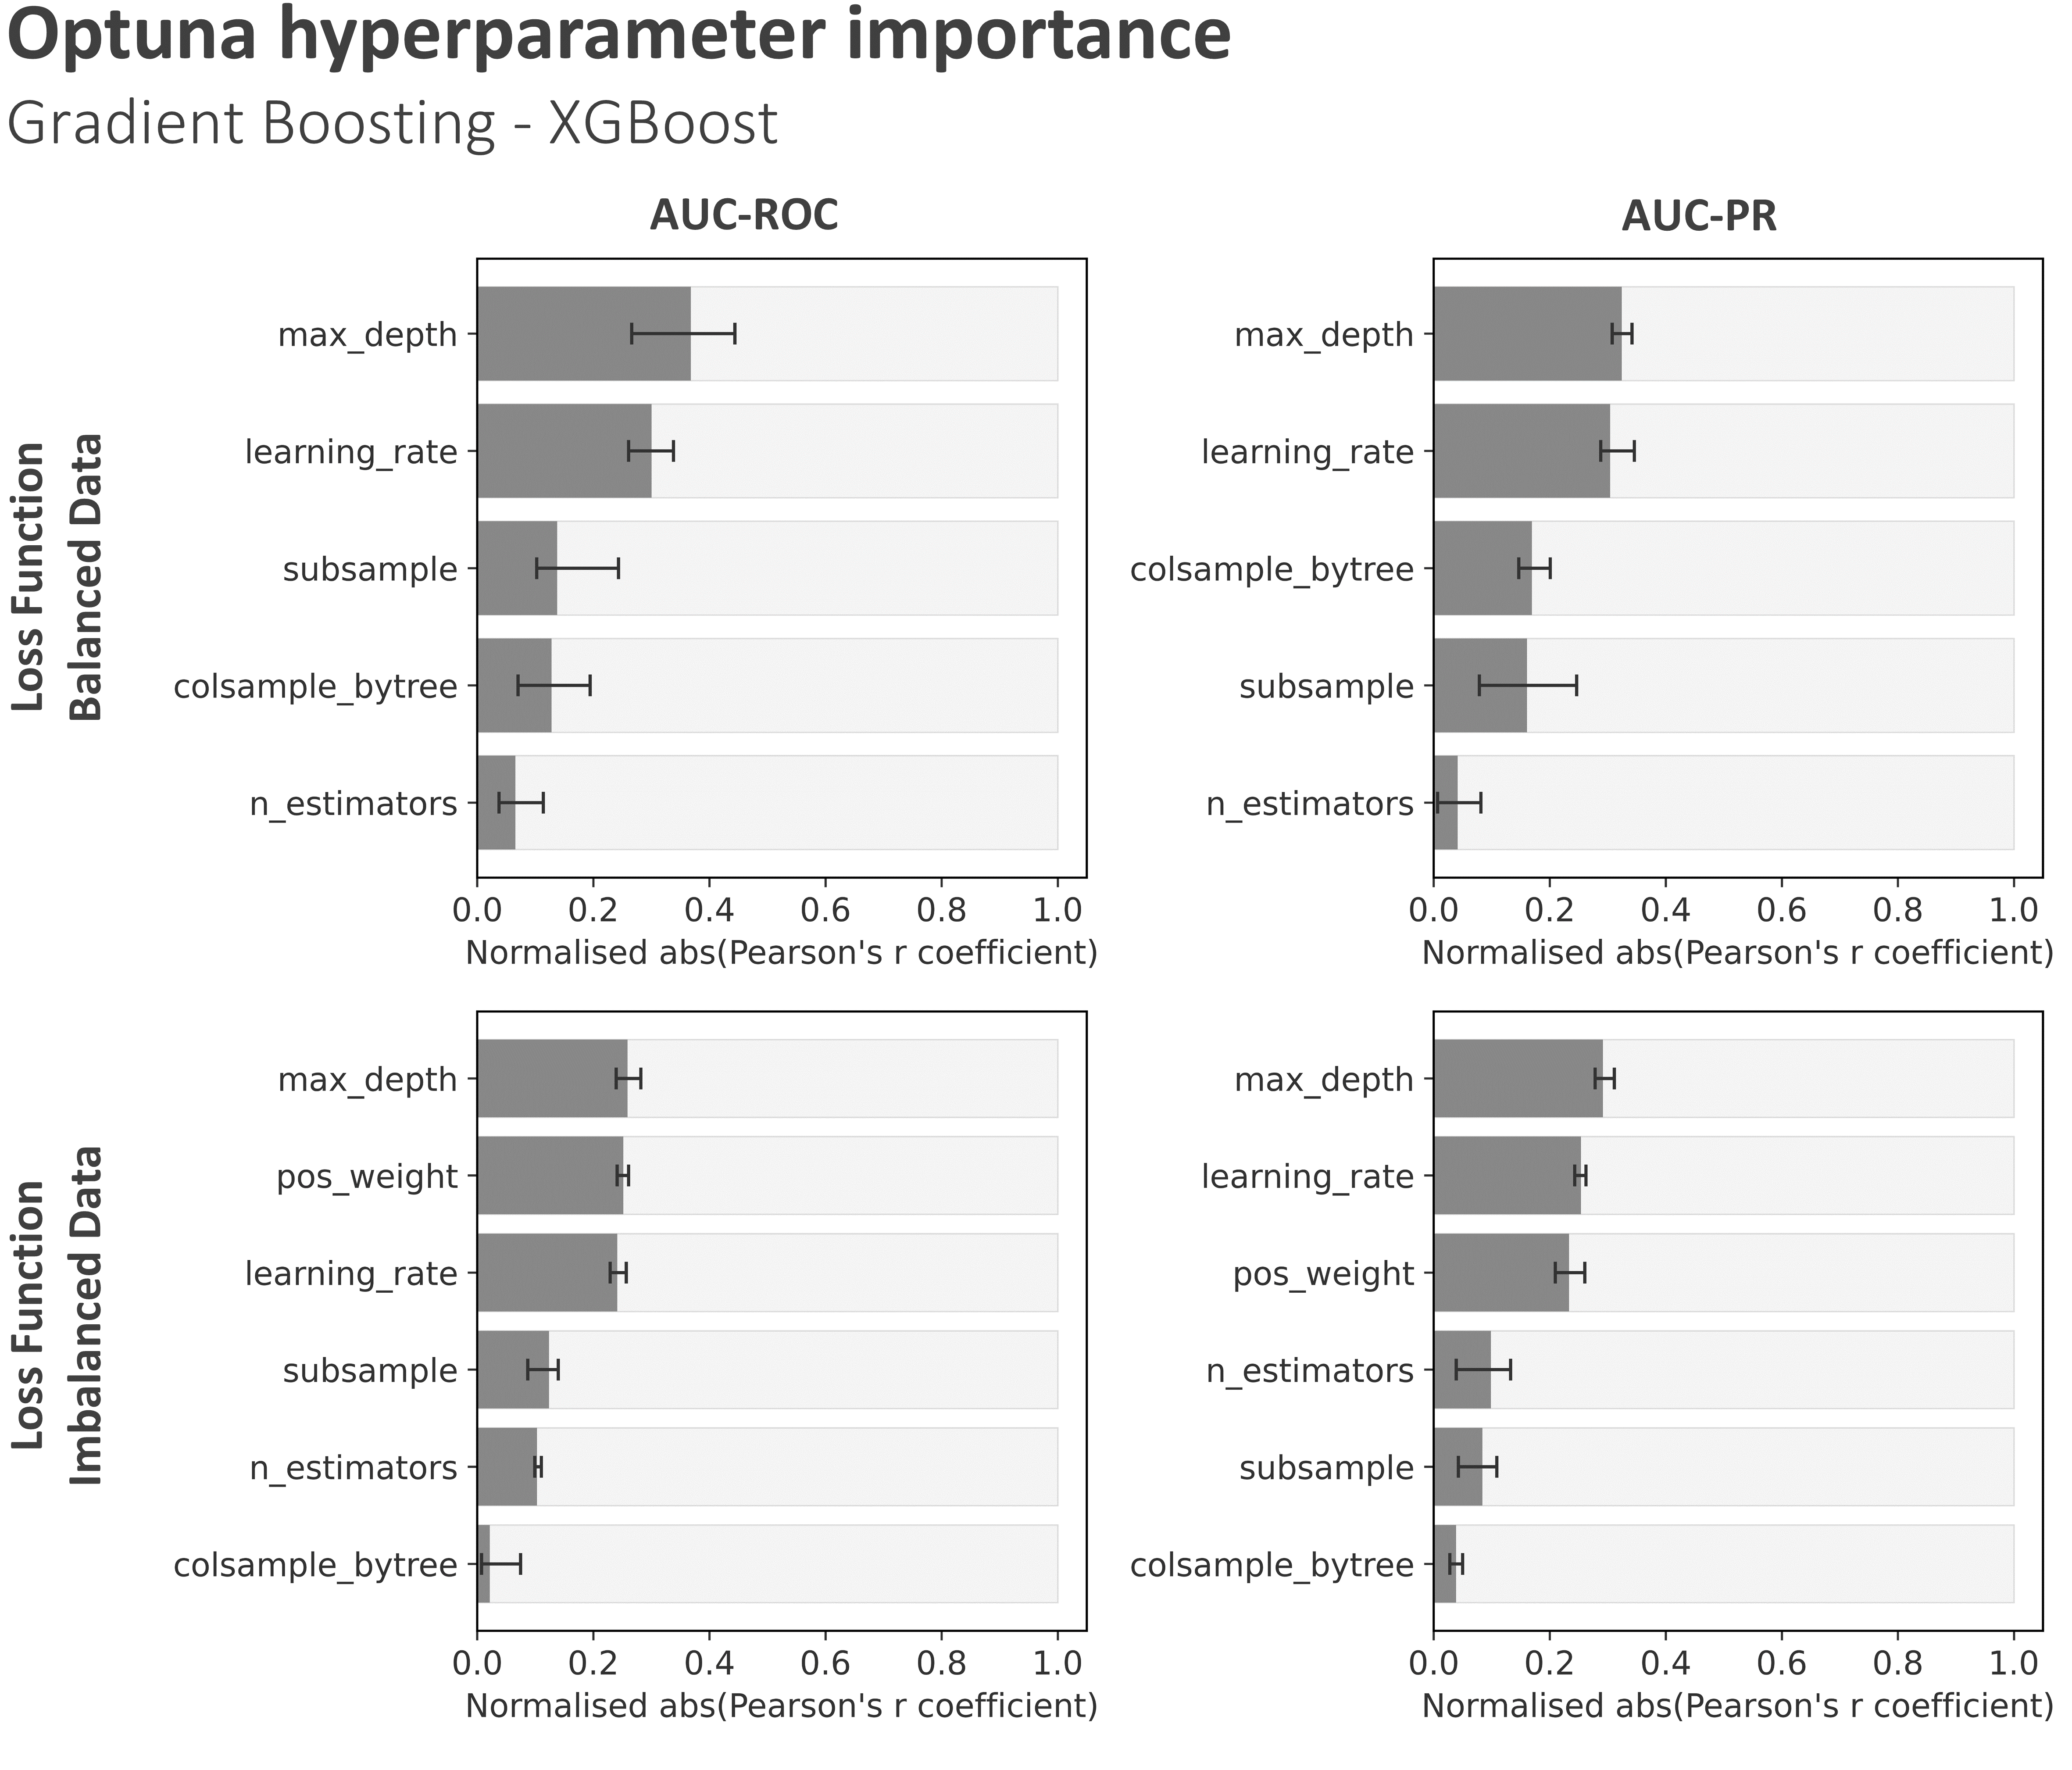
\includegraphics[scale=0.9]{optuna_parameters_importance_gradient_boosting_xgboost.png}
\caption{\textbf{Optuna's hyperparameter importance for the XGBoost implementation of gradient boosting.} Normalised absolute Pearson's correlation coefficients obtained for the n\_trials = 20 trials run over the \textcolor{colourInnerTraining}{\textit{inner training folds}} (bars represent mean values, whilst error bars show the minimum and maximum values across the Optuna trials). Feature importance is shown for models trained with loss functions for balanced datasets and specific for imbalanced datasets, and for both evaluation metrics (AUC-ROC and AUC-PR).}
\label{fig:optuna_parameters_importance_gradient_boosting_xgboost}
\end{figure}

\begin{figure}[htbp]
\centering
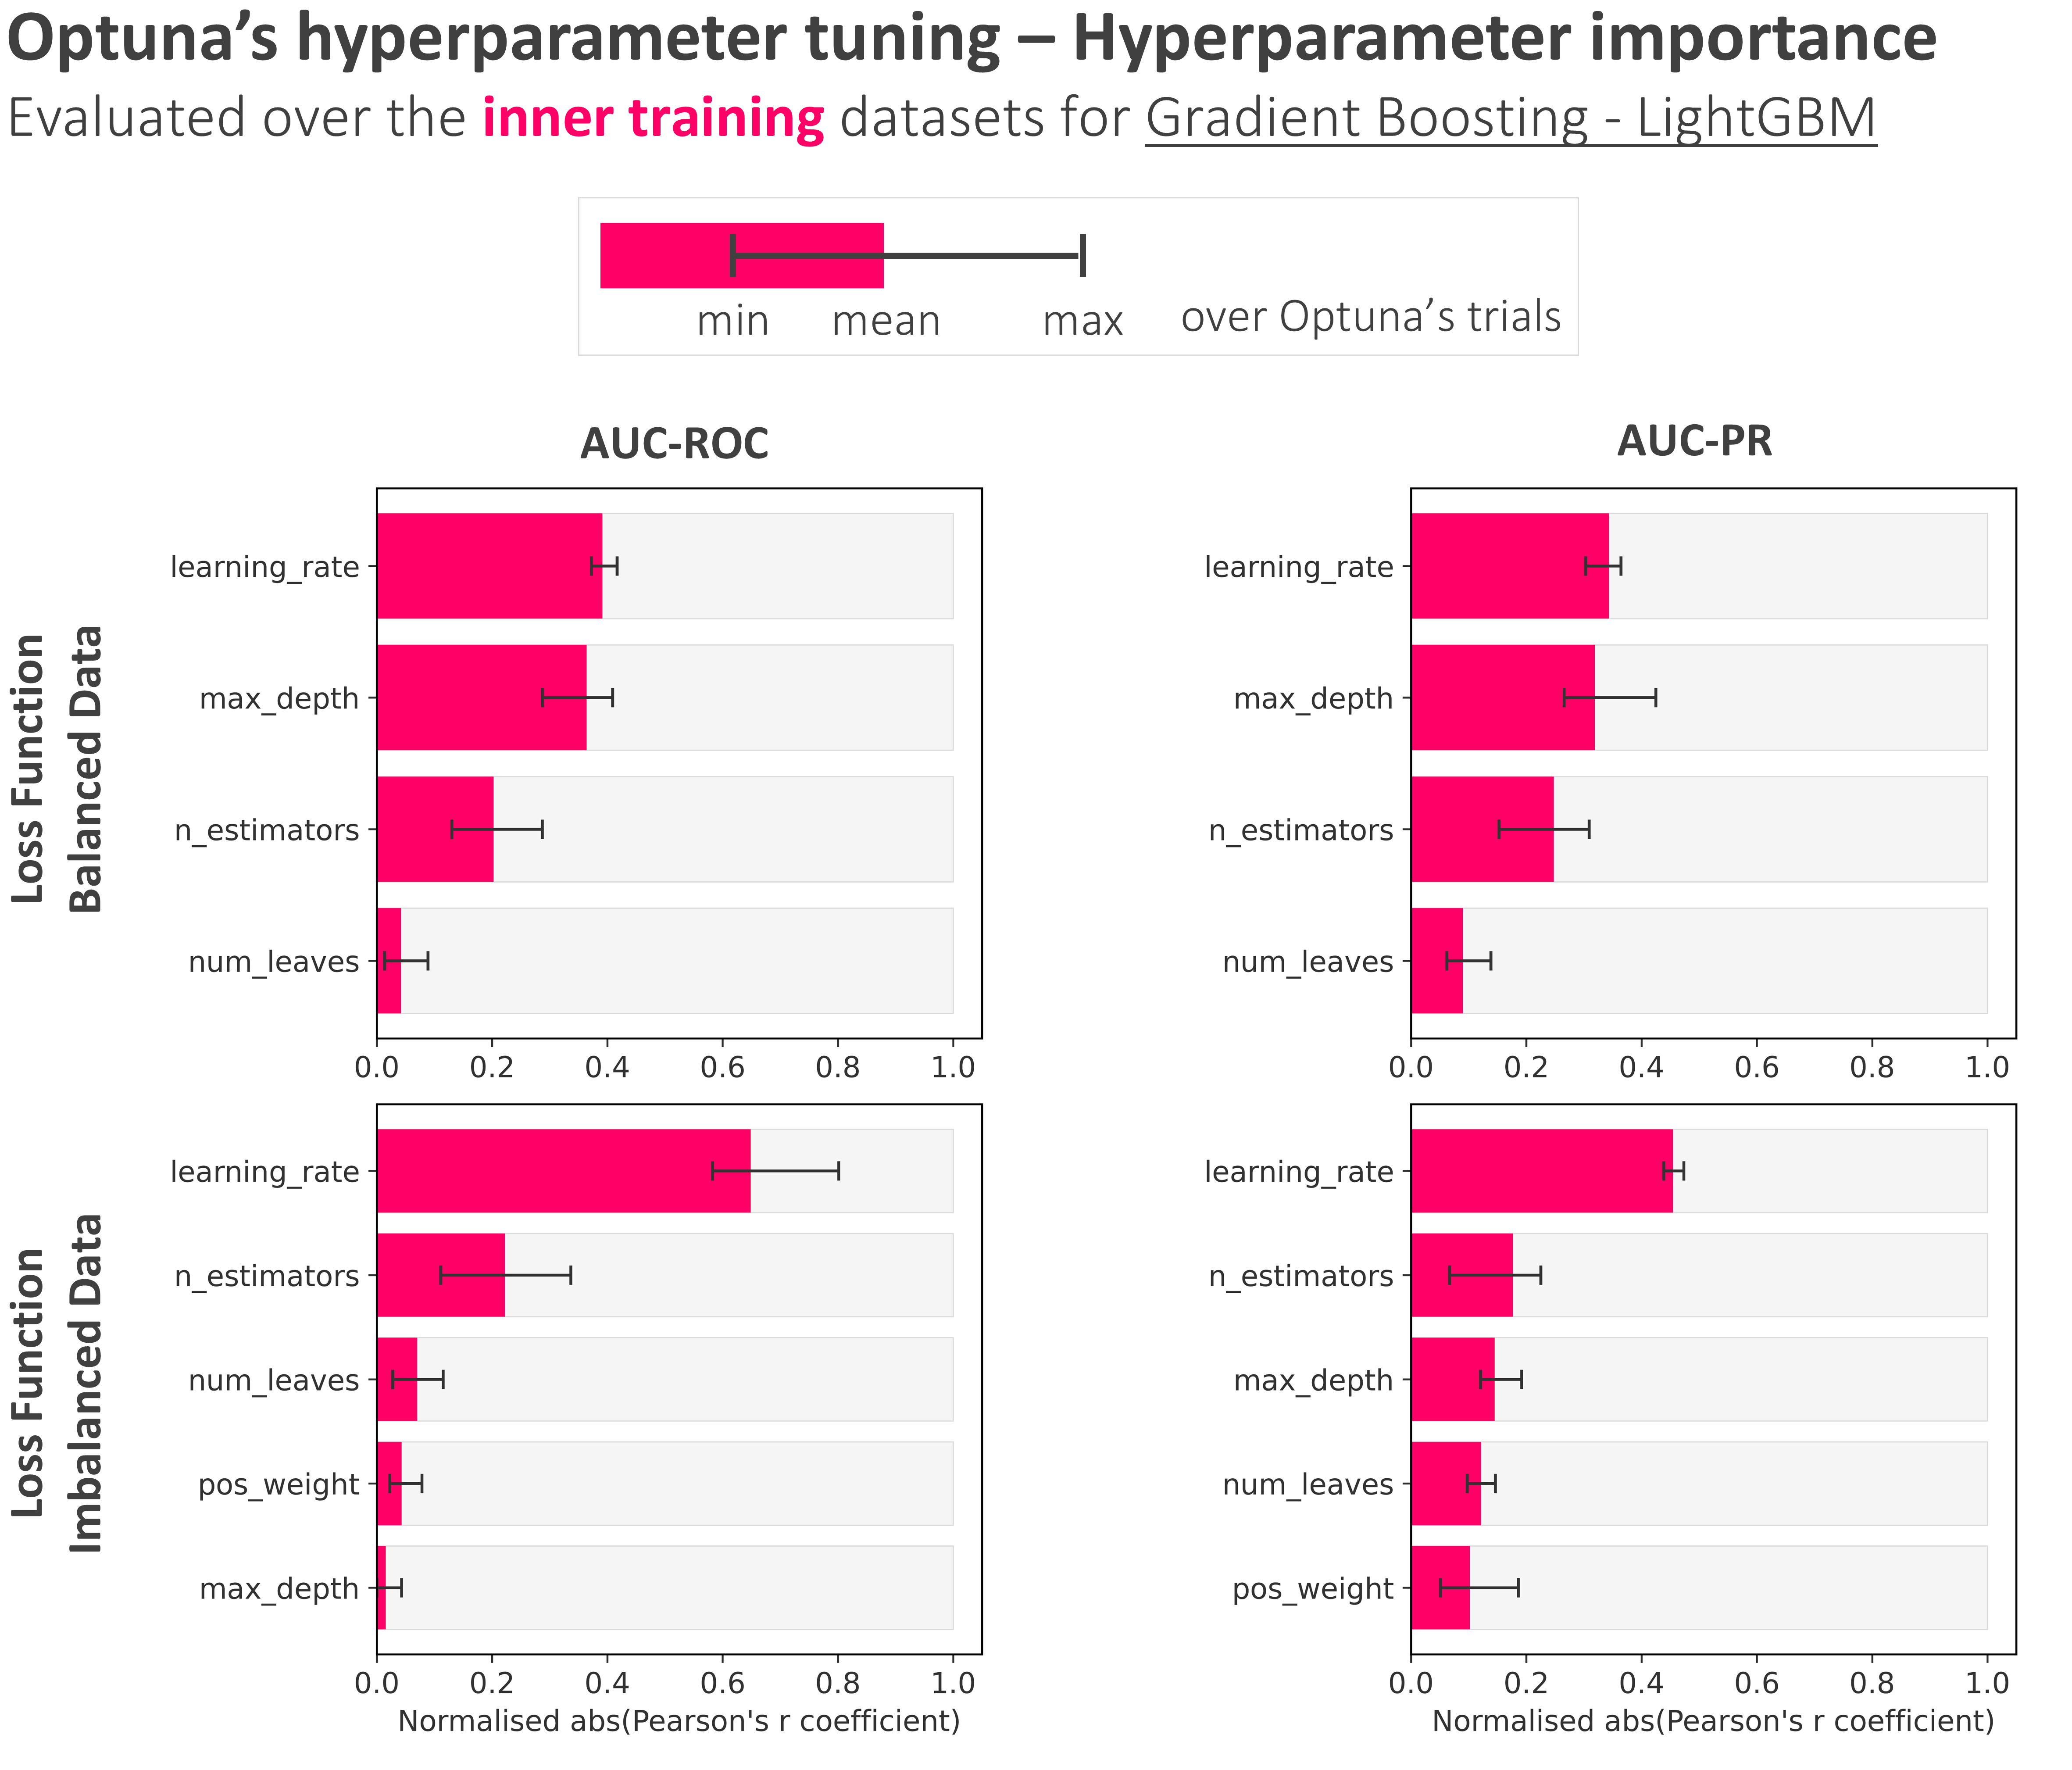
\includegraphics[scale=0.9]{optuna_parameters_importance_gradient_boosting_lightgbm.png}
\caption{\textbf{Optuna's hyperparameter importance for the LightGBM implementation of gradient boosting.} Similar to Figure \ref{fig:optuna_parameters_importance_gradient_boosting_xgboost}}.
\label{fig:optuna_parameters_importance_gradient_boosting_lightgbm}
\end{figure}

\begin{figure}[htbp]
\centering
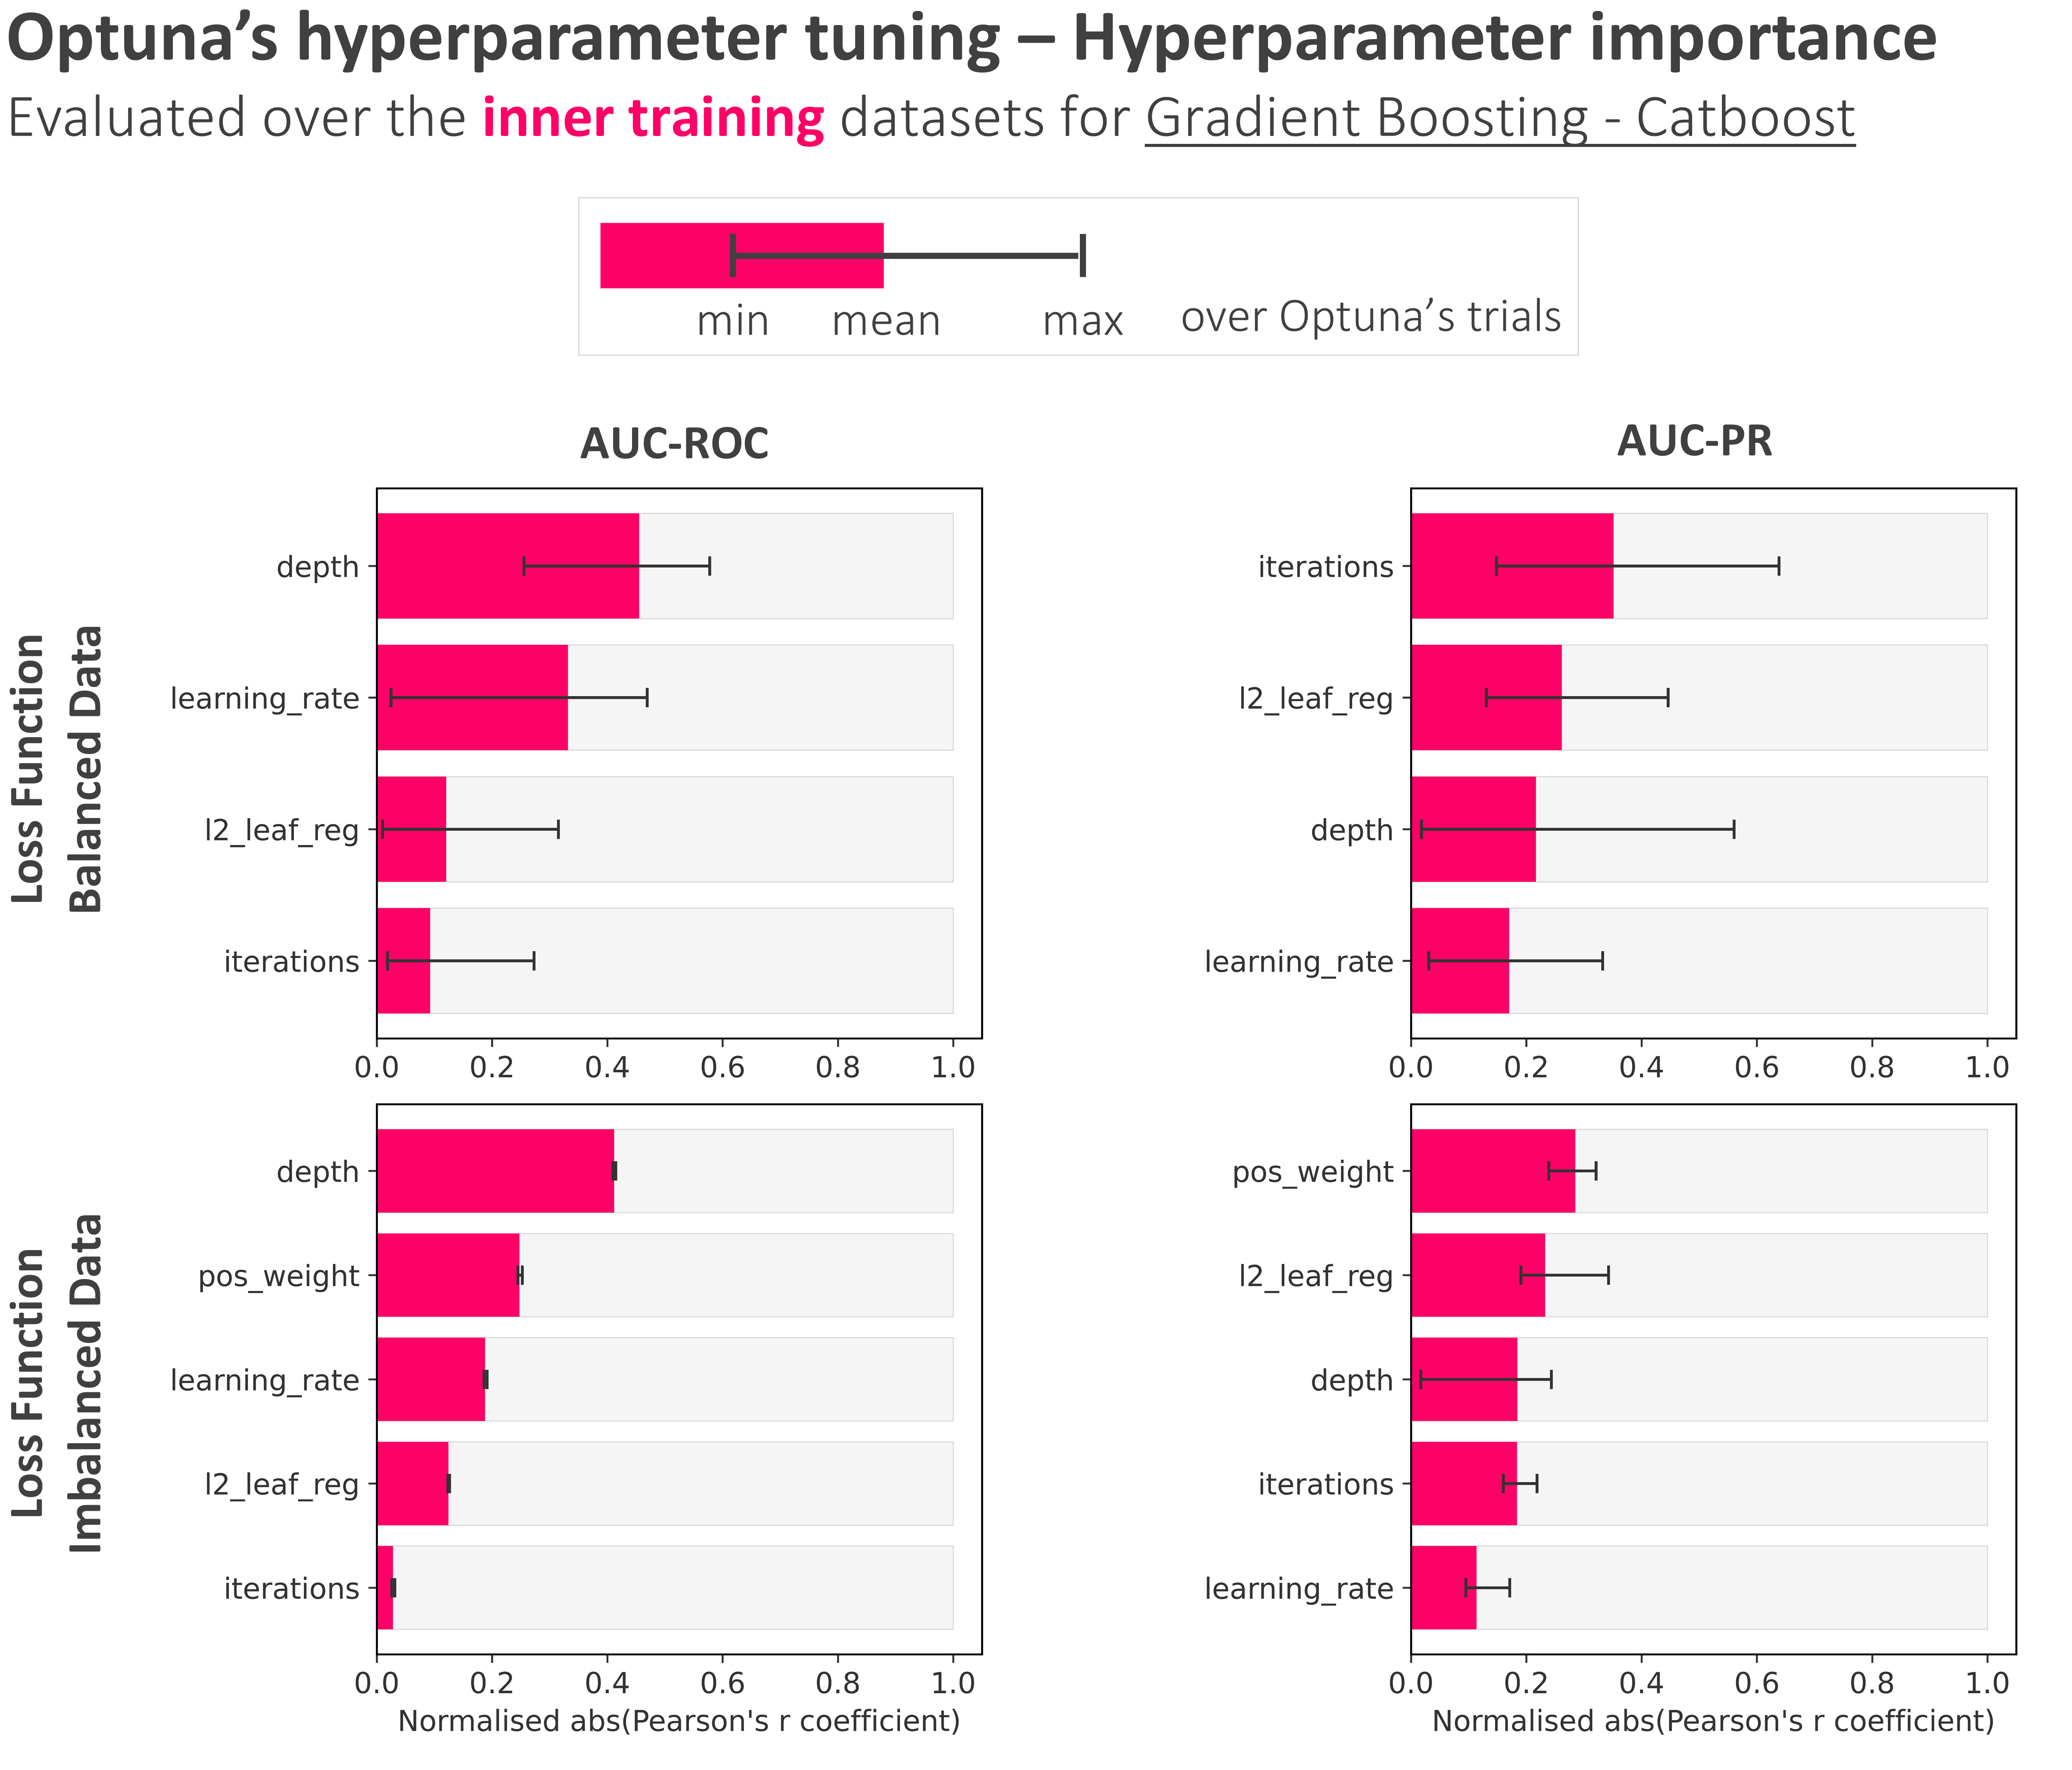
\includegraphics[scale=0.9]{optuna_parameters_importance_gradient_boosting_catboost.png}
\caption{\textbf{Optuna's hyperparameter importance for the CatBoost implementation of gradient boosting.} Similar to Figure \ref{fig:optuna_parameters_importance_gradient_boosting_xgboost}}.
\label{fig:optuna_parameters_importance_gradient_boosting_catboost}
\end{figure}

In contrast \marginpara{Hyperparameter importance: random forest implementations} to gradient boosting implementations, random forest models exhibit inconsistent hyperparameter importance rankings across different loss functions and evaluation metrics, with parameters such as maximum depth, feature sampling ratios, and the number of estimators alternating in their relative influence depending on whether AUC-ROC or AUC-PR is optimised. This variability suggests that random forest hyperparameter spaces possess multiple viable configurations that achieve similar performance through different mechanisms (some configurations may excel through deeper individual trees, whilst others compensate with more aggressive feature sampling or a larger ensemble size), making the optimisation landscape more flexible but potentially more challenging to navigate systematically.

\begin{figure}[htbp]
\centering
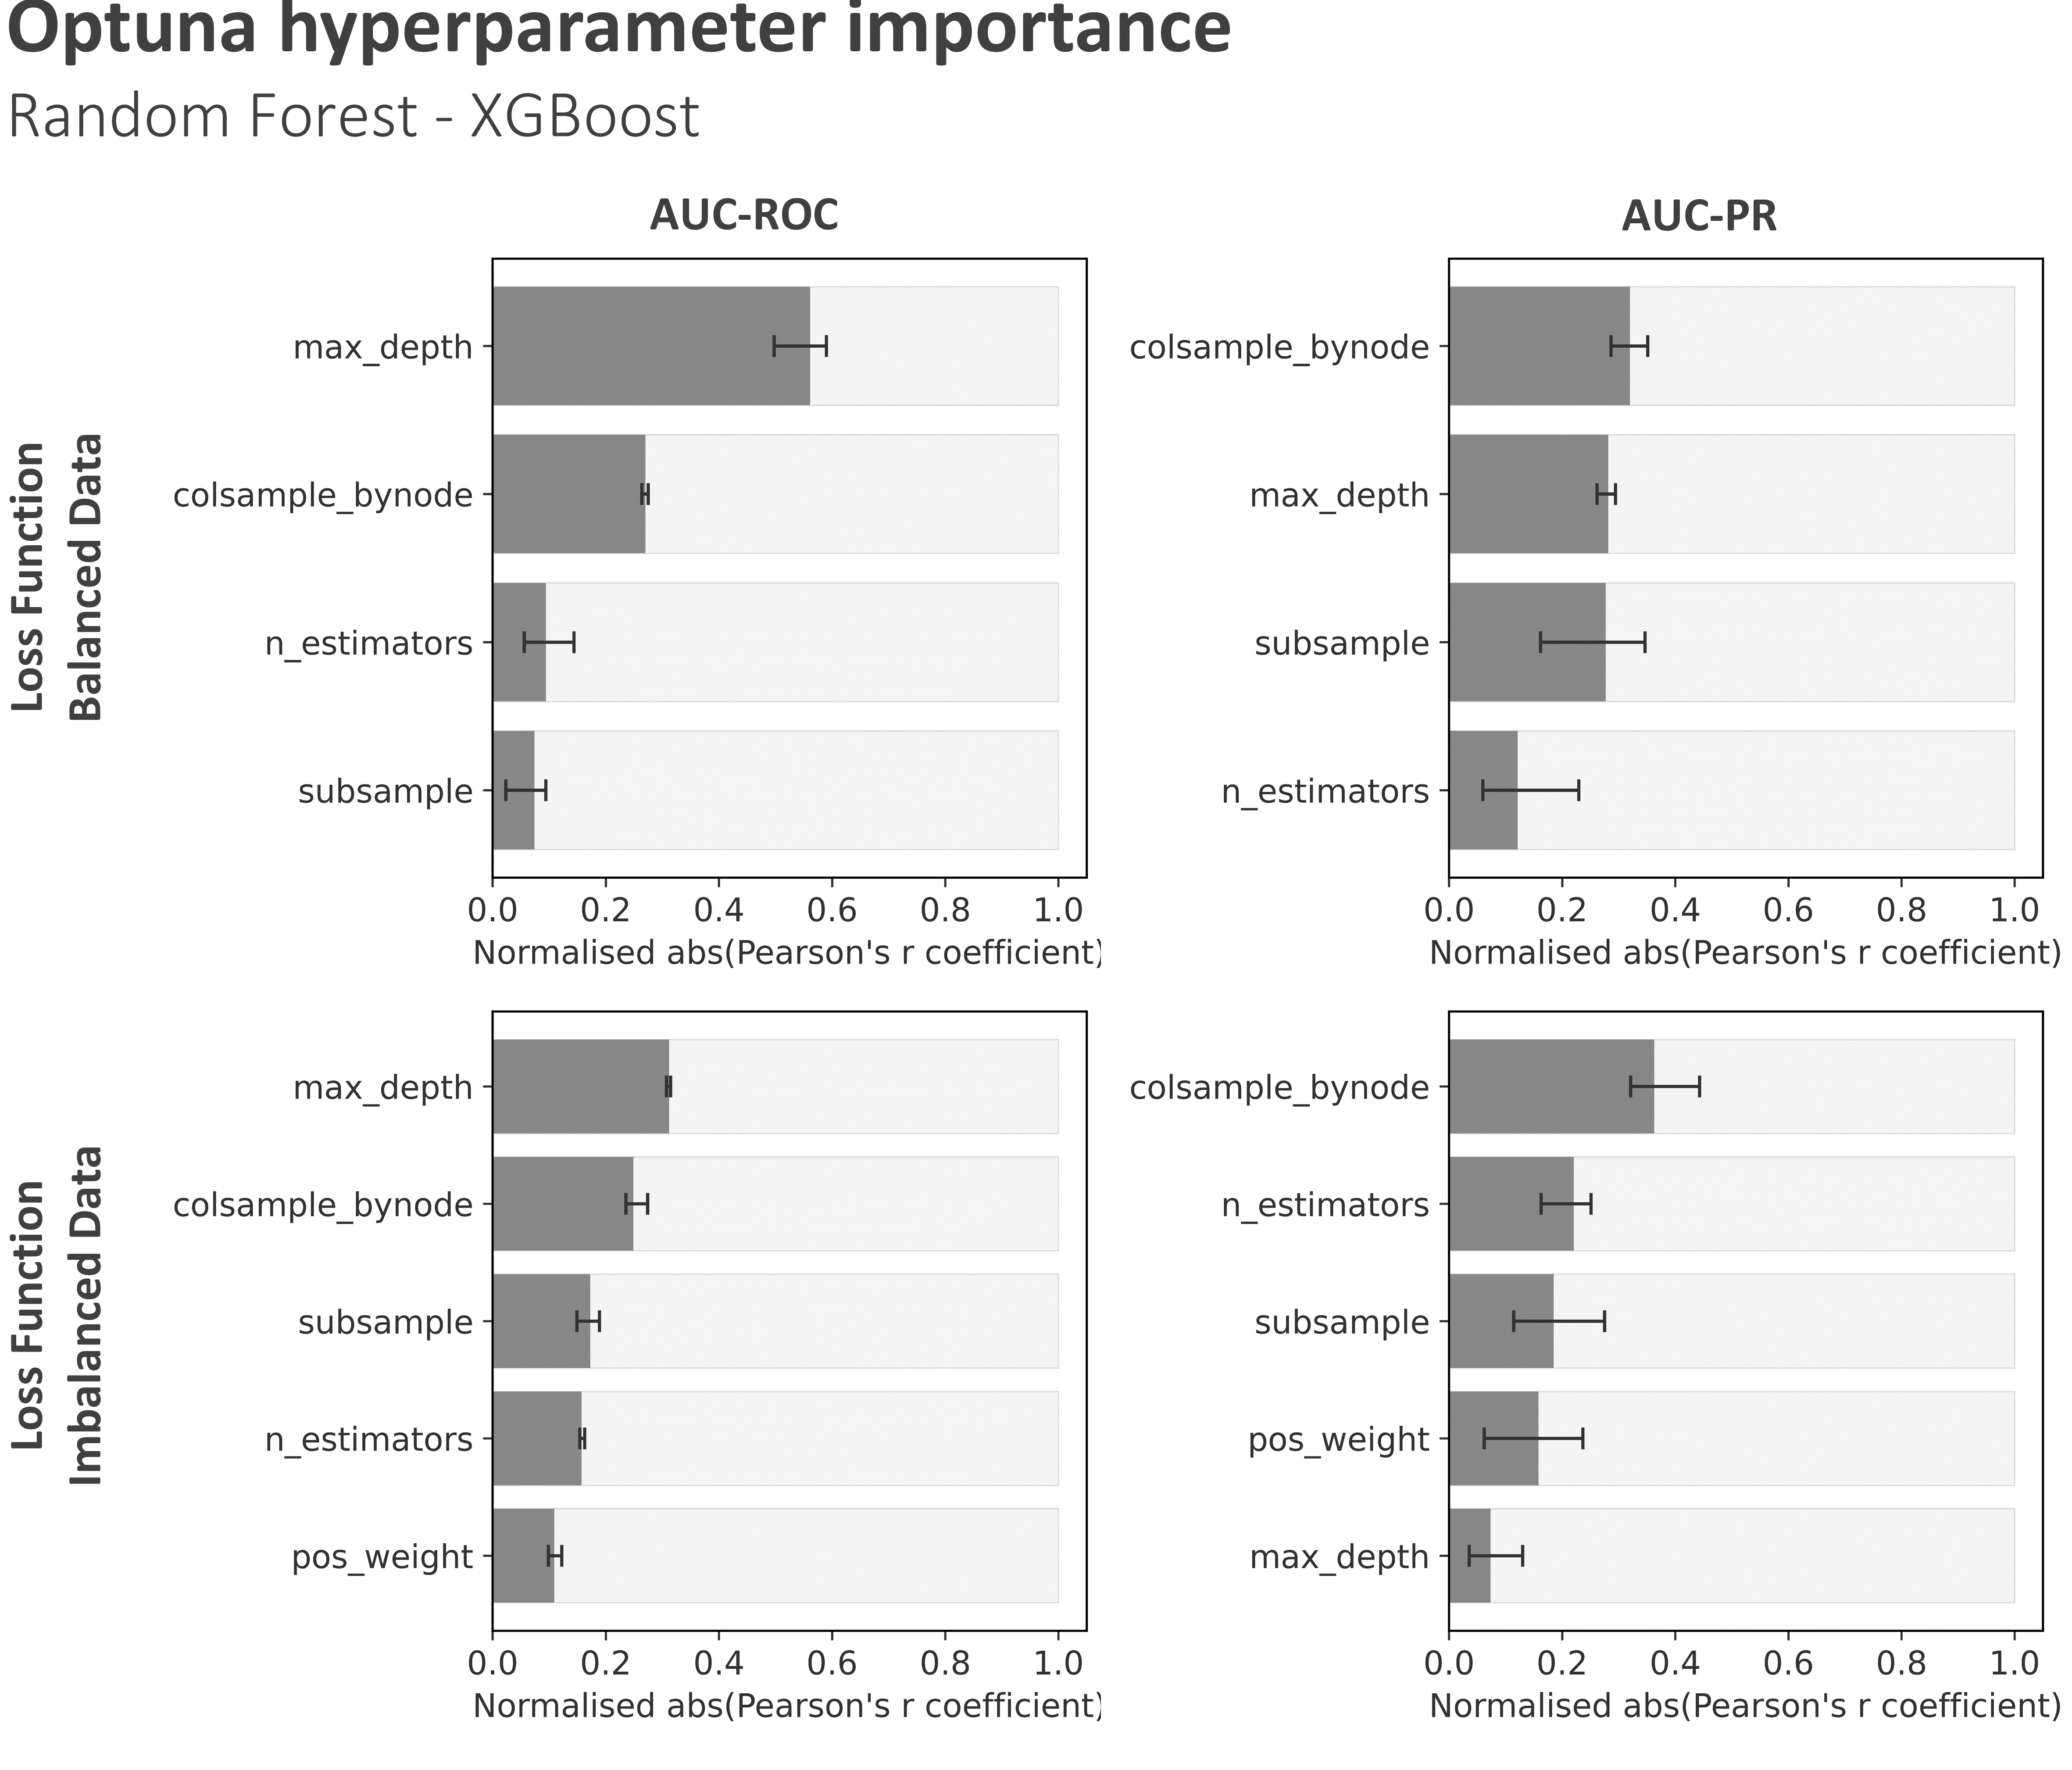
\includegraphics[scale=0.9]{optuna_parameters_importance_random_forest_xgboost.png}
\caption{\textbf{Optuna's hyperparameter importance for the XGBoost implementation of random forest.} Similar to Figure \ref{fig:optuna_parameters_importance_gradient_boosting_xgboost}}.
\label{fig:optuna_parameters_importance_random_forest_xgboost}
\end{figure}

\begin{figure}[htbp]
\centering
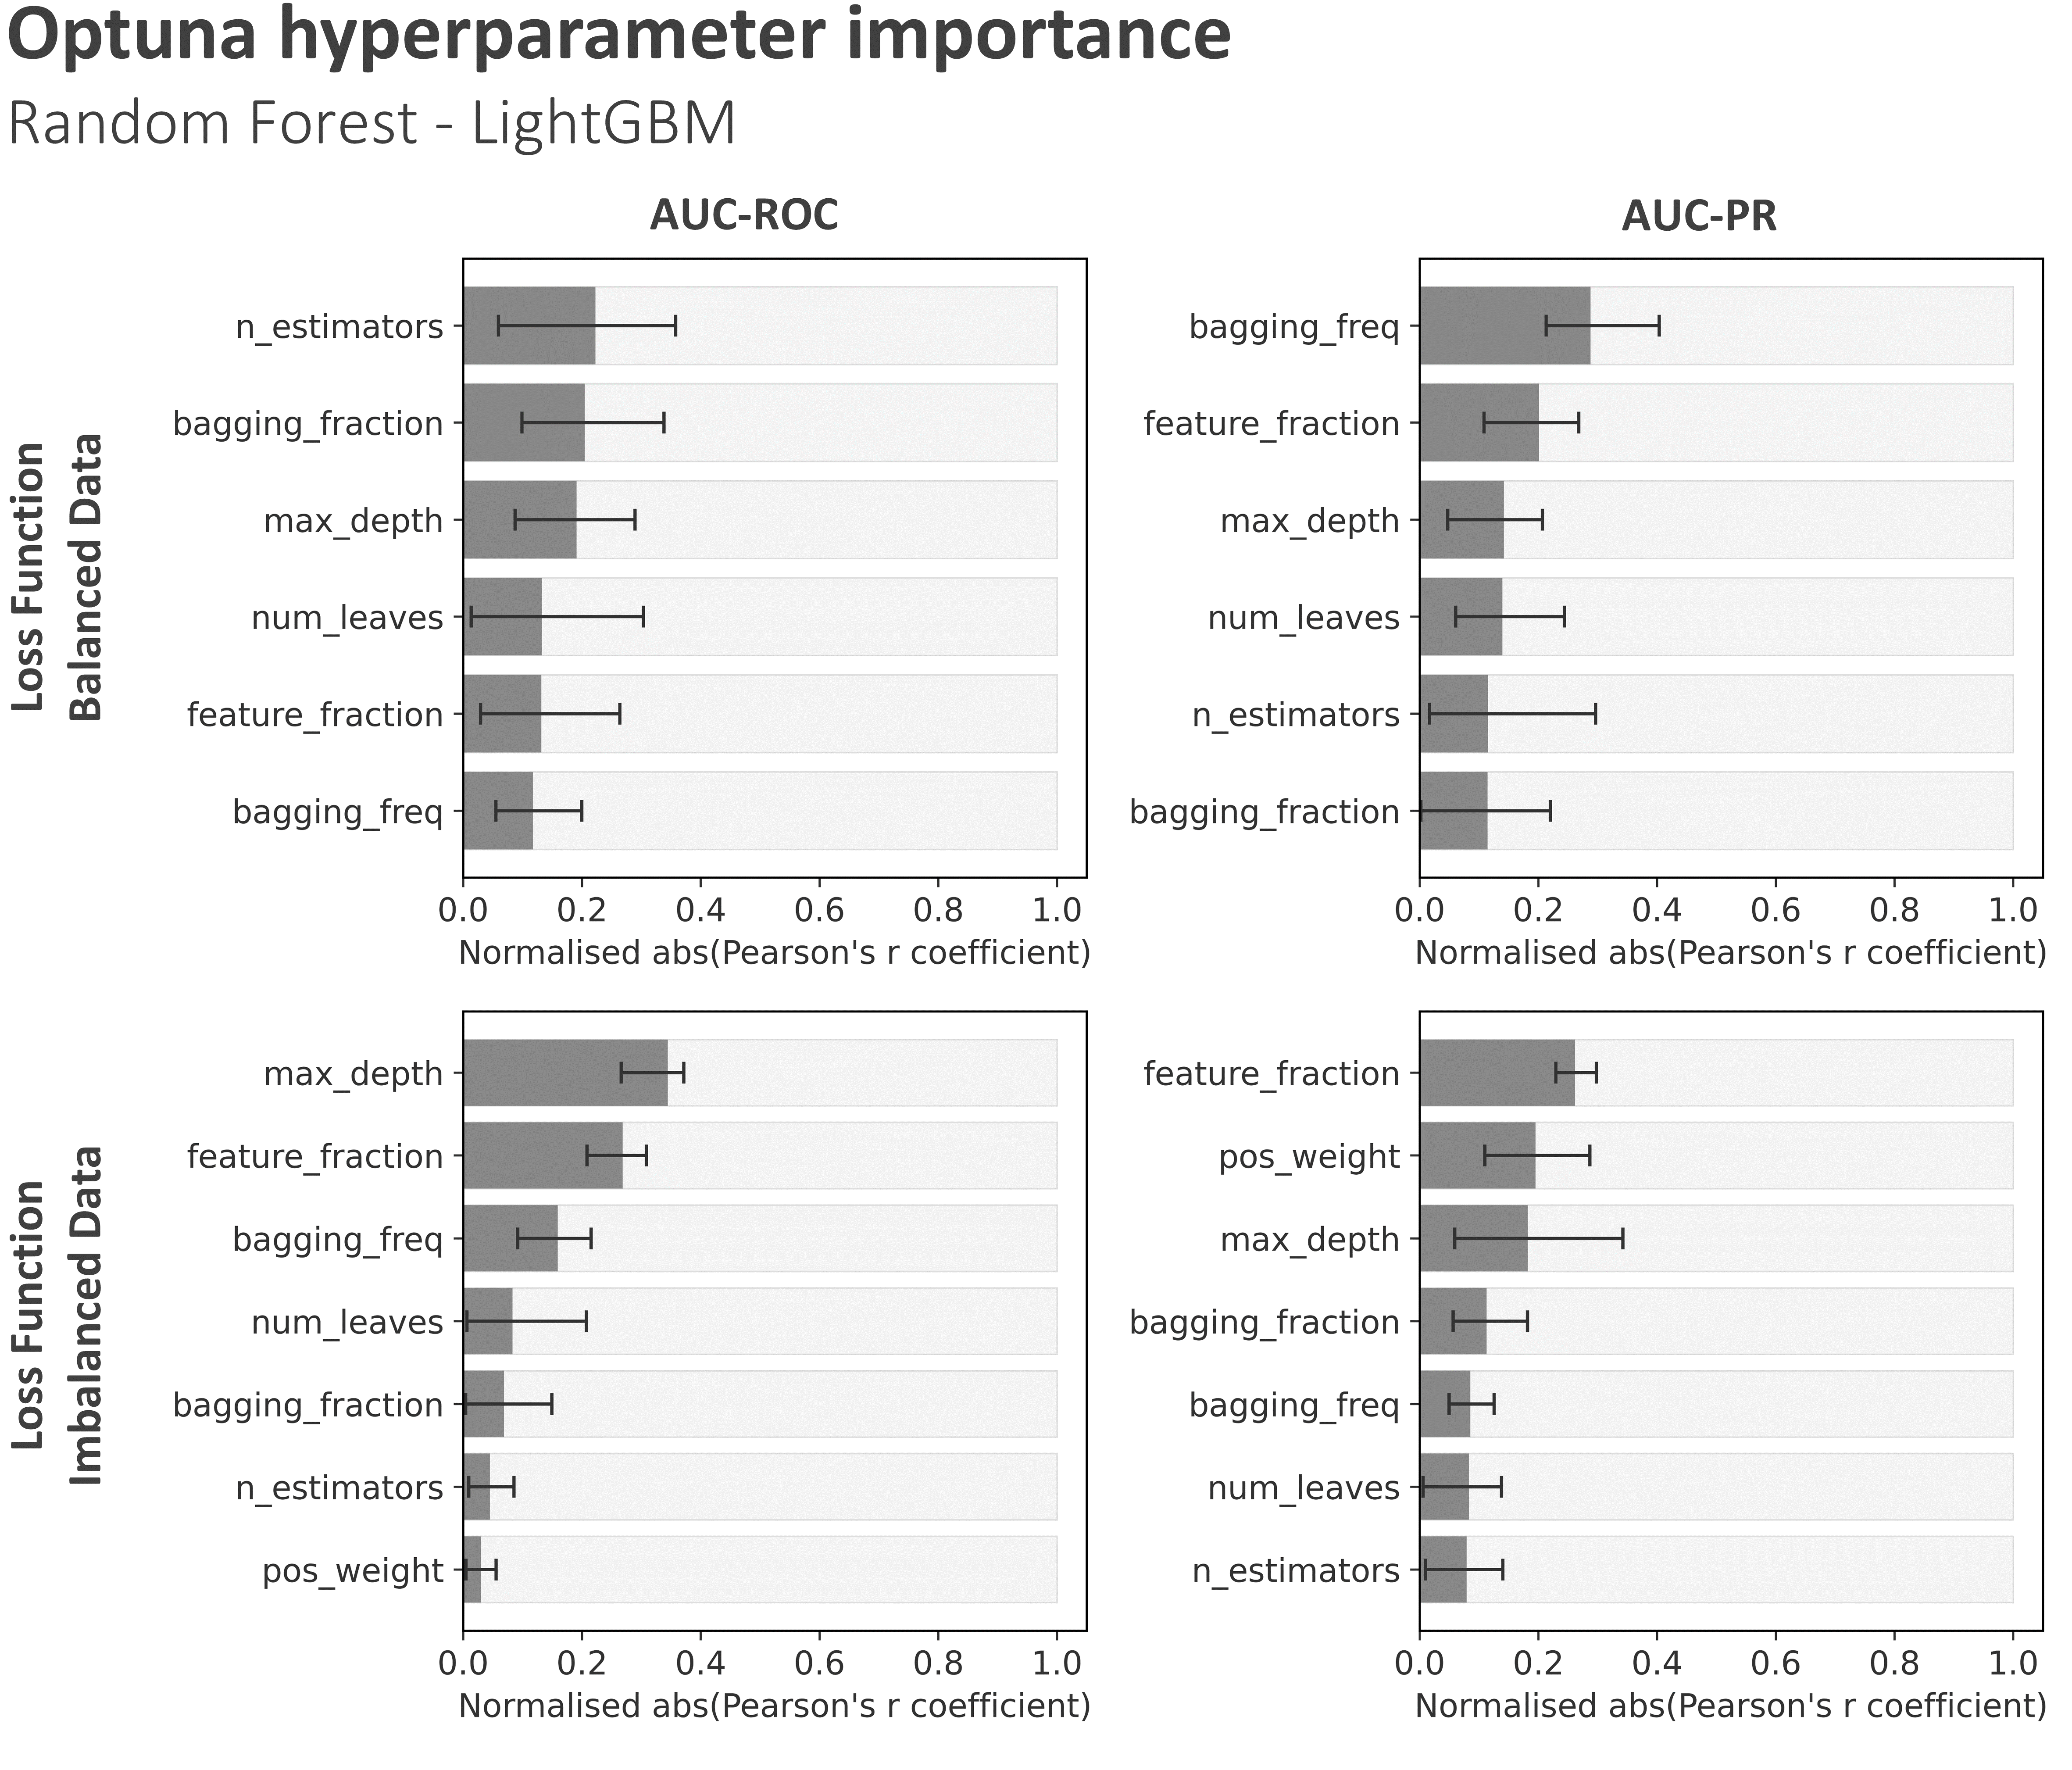
\includegraphics[scale=0.9]{optuna_parameters_importance_random_forest_lightgbm.png}
\caption{\textbf{Optuna's hyperparameter importance for the LightGBM implementation of random forest.} Similar to Figure \ref{fig:optuna_parameters_importance_gradient_boosting_xgboost}}.
\label{fig:optuna_parameters_importance_random_forest_lightgbm}
\end{figure}

The \marginpara{Hyperparameter importance: feed-forward neural networks} dominance of units\_0, dropout\_0, and learning rate for neural networks suggests that performance is primarily determined by the configuration of the first hidden layer, rather than the overall network depth. The parameter units\_0 controls the initial representational capacity, determining how effectively raw hydro-meteorological features are transformed into meaningful intermediate representations for detecting rare flash flood patterns. This layer must balance sufficient complexity to capture non-linear relationships whilst avoiding overfitting to the sparse positive examples. The high importance of dropout\_0 demonstrates that regularisation at this critical layer is essential for generalisation under extreme class imbalance. By randomly deactivating neurons during training, dropout forces the development of robust, redundant representations that prevent the model from memorising noise in the limited positive examples. The prominence of the learning rate parameter reflects the challenge of navigating an imbalanced dataset, where the gradient signal from rare positive examples can be easily overwhelmed by the abundance of negative cases. The diminished importance of deeper layer parameters suggests that shallow, well-regularised architectures may be the best choice for this application.

\begin{figure}[htbp]
\centering
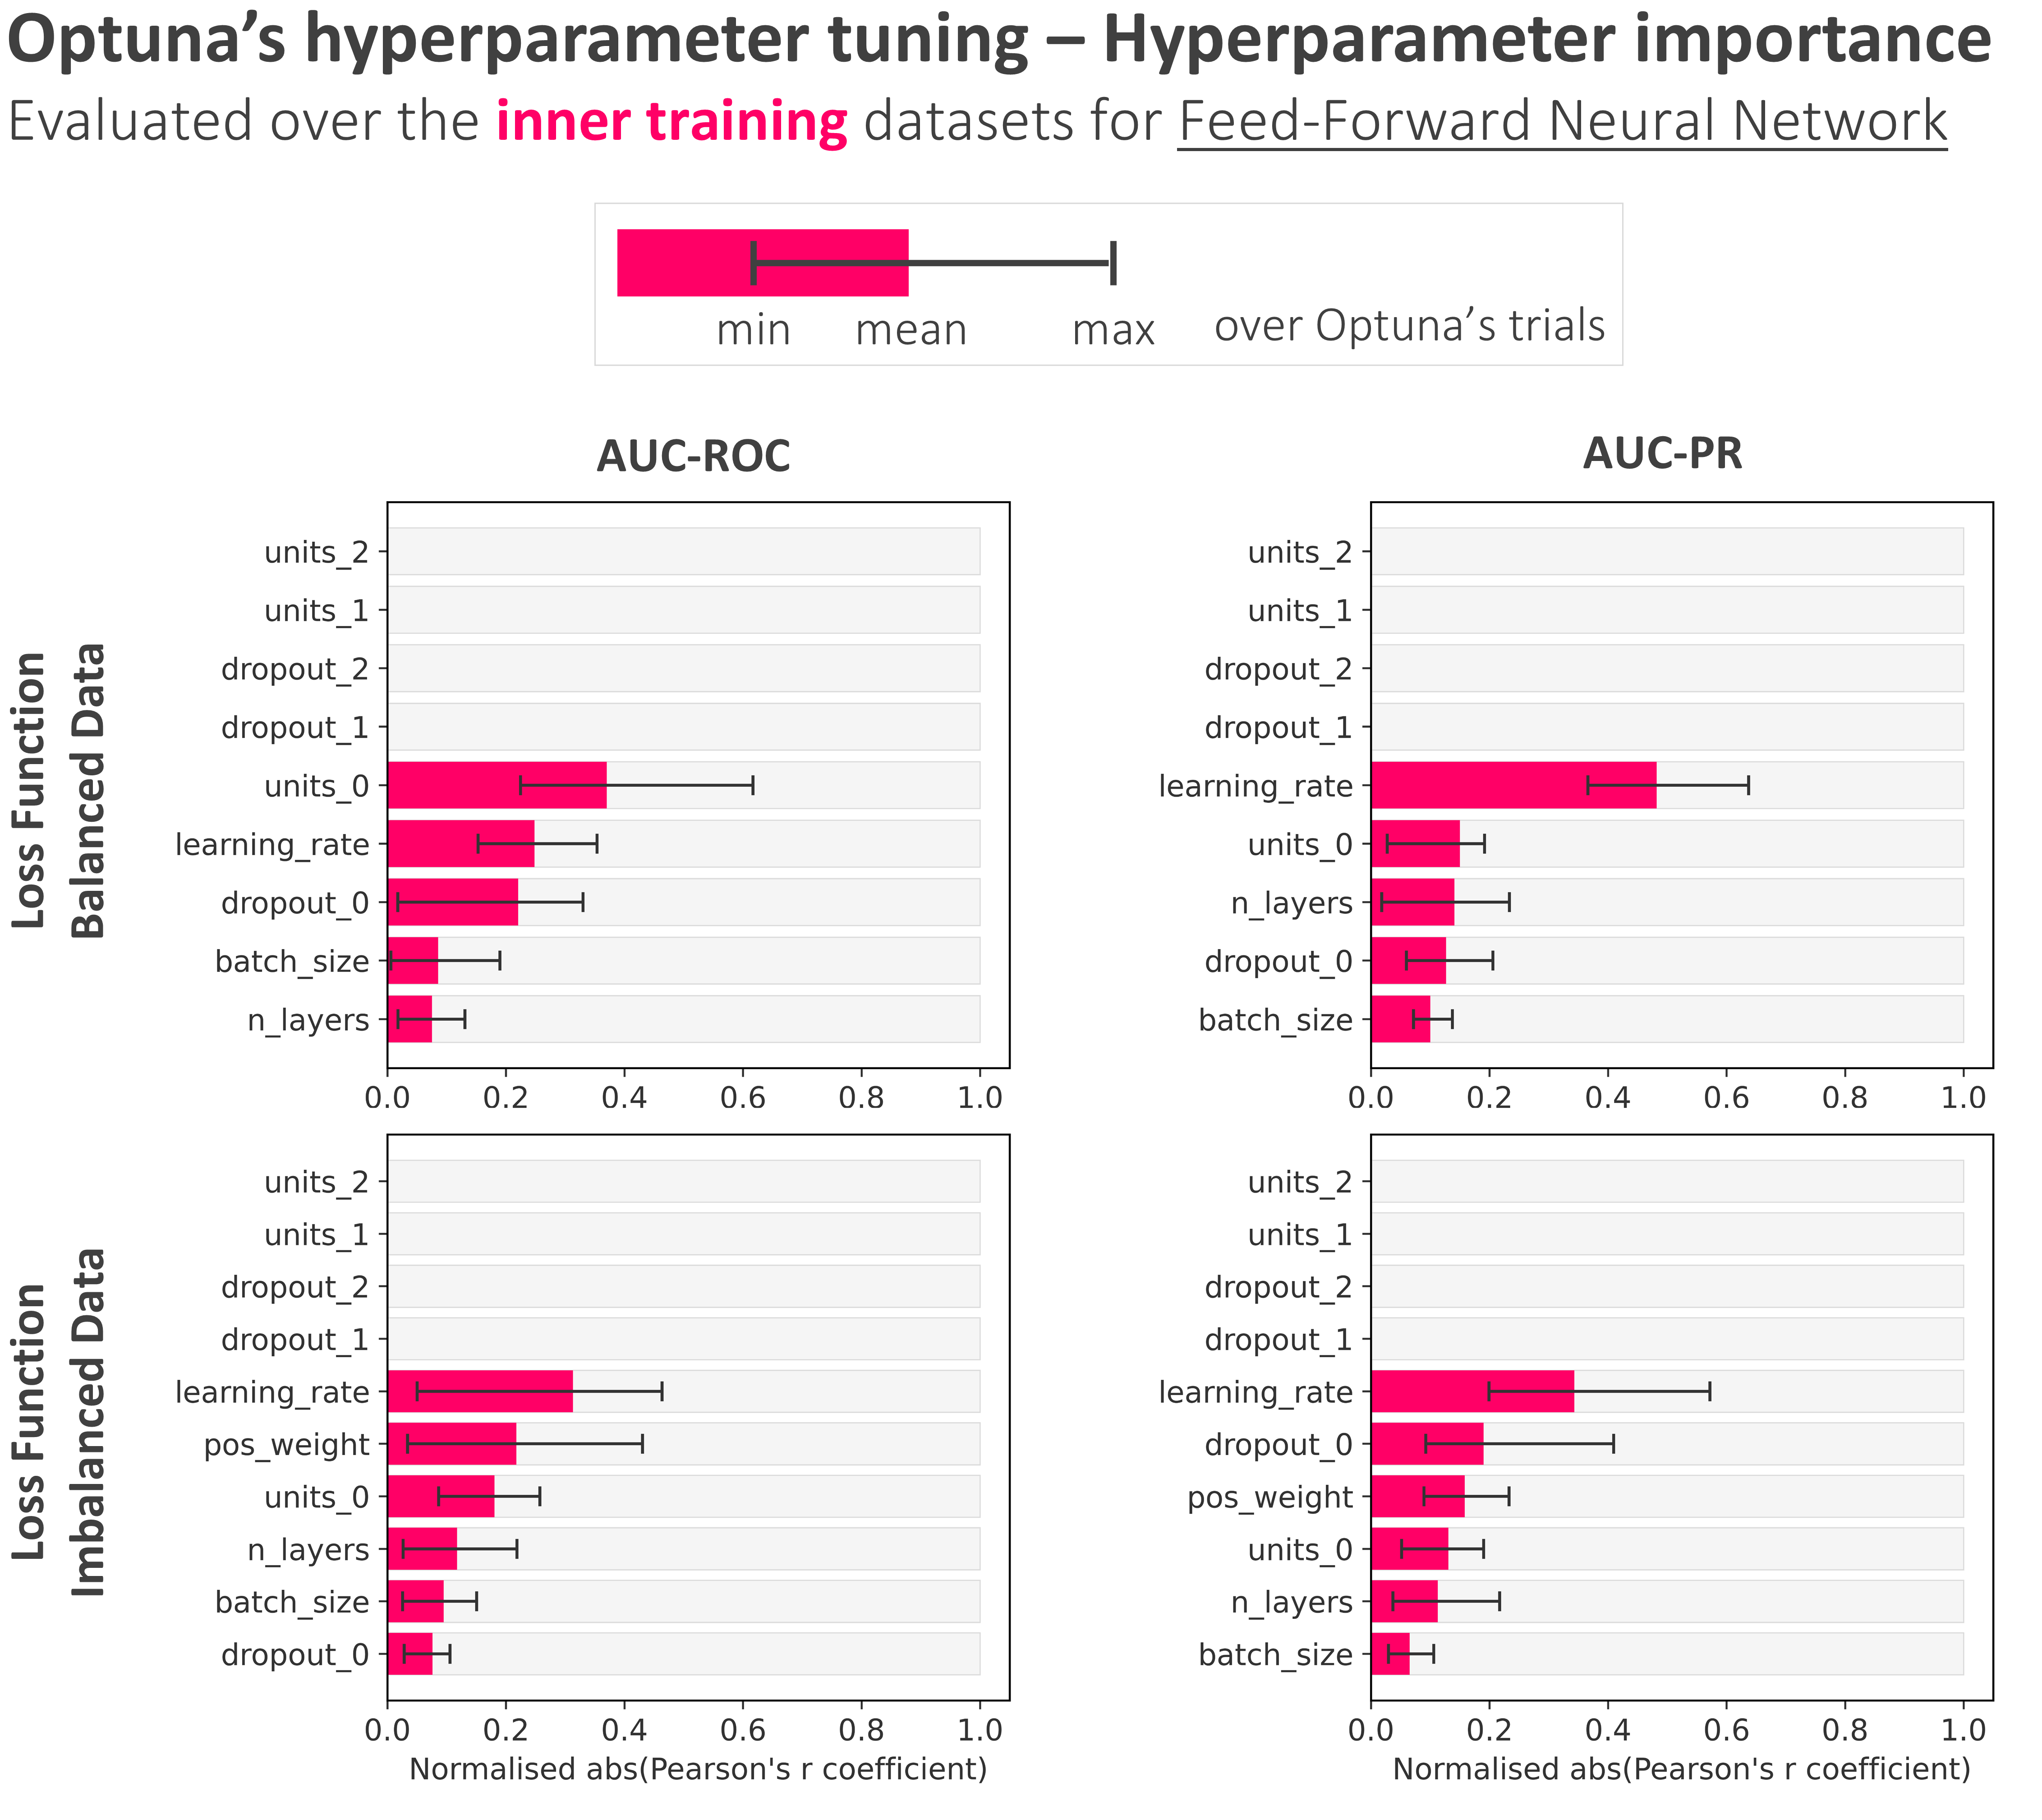
\includegraphics[scale=0.9]{optuna_parameters_importance_feed_forward_nn.png}
\caption{\textbf{Optuna's hyperparameter importance for feed-forward neural network.} Similar to Figure \ref{fig:optuna_parameters_importance_gradient_boosting_xgboost}}.
\label{fig:optuna_parameters_importance_feed_forward_nn}
\end{figure}


\subsection{Verification results over reanalysis data}

To assess the generalisation capabilities of the trained data-driven models, this section compares various performance metrics (presented in Section \ref{data_driven_flash_floods_short_medium_range_methods_verif_scores}) between the \textcolor{colourTraining}{training dataset}, with data from 2001 to 2020, and the independent 
\textcolor{colourTest}{verification dataset}, with data from 2021 to 2024.

All \marginpara{Verification results over reanalysis data: overall scores (AUC-ROC, AUC-PR, and FB)} data-driven models exhibit relatively stable AUC-ROC values around 0.8 for the \textcolor{colourTest}{verification dataset} with minimal decrease from the AUC-ROC values obtained for the \textcolor{colourTraining}{training dataset} (Figure \ref{fig:verif_training_test_overall}, first column). This behaviour is constant across both evaluation metrics (AUC-ROC and AUC-PR) and both types of loss function (general for balanced datasets and specific for imbalanced datasets). Hence, all data-driven models show an overall discrimination ability that generalises well from training to verification datasets. The AUC-PR values demonstrate more variability across data-driven models (Figure \ref{fig:verif_training_test_overall}, second column), with CatBoost showing the highest estimates overall, especially when hyperparameters are tuned maximising the AUC-ROC evaluation metric (for both types of loss function). For all models, however, values of AUC-PR remain relatively small (Close to 0). Even though all models show a tendency to slightly overestimate the frequency of areas at risk of flash flood (FB just above 1, Figure \ref{fig:verif_training_test_overall}, third column), the FB values also show high variability across the data-driven models. When considering the generic loss function, the XGBoost and LightGBM implementations for random forest and gradient boosting obtain the closest values to 1, but increase of ~20\% when considering the loss function specific for imbalanced datasets, showing even greater FB than the other tested models (which maintain similar values than those obtained when considering the generic loss function).

\begin{figure}[htbp]
\centering
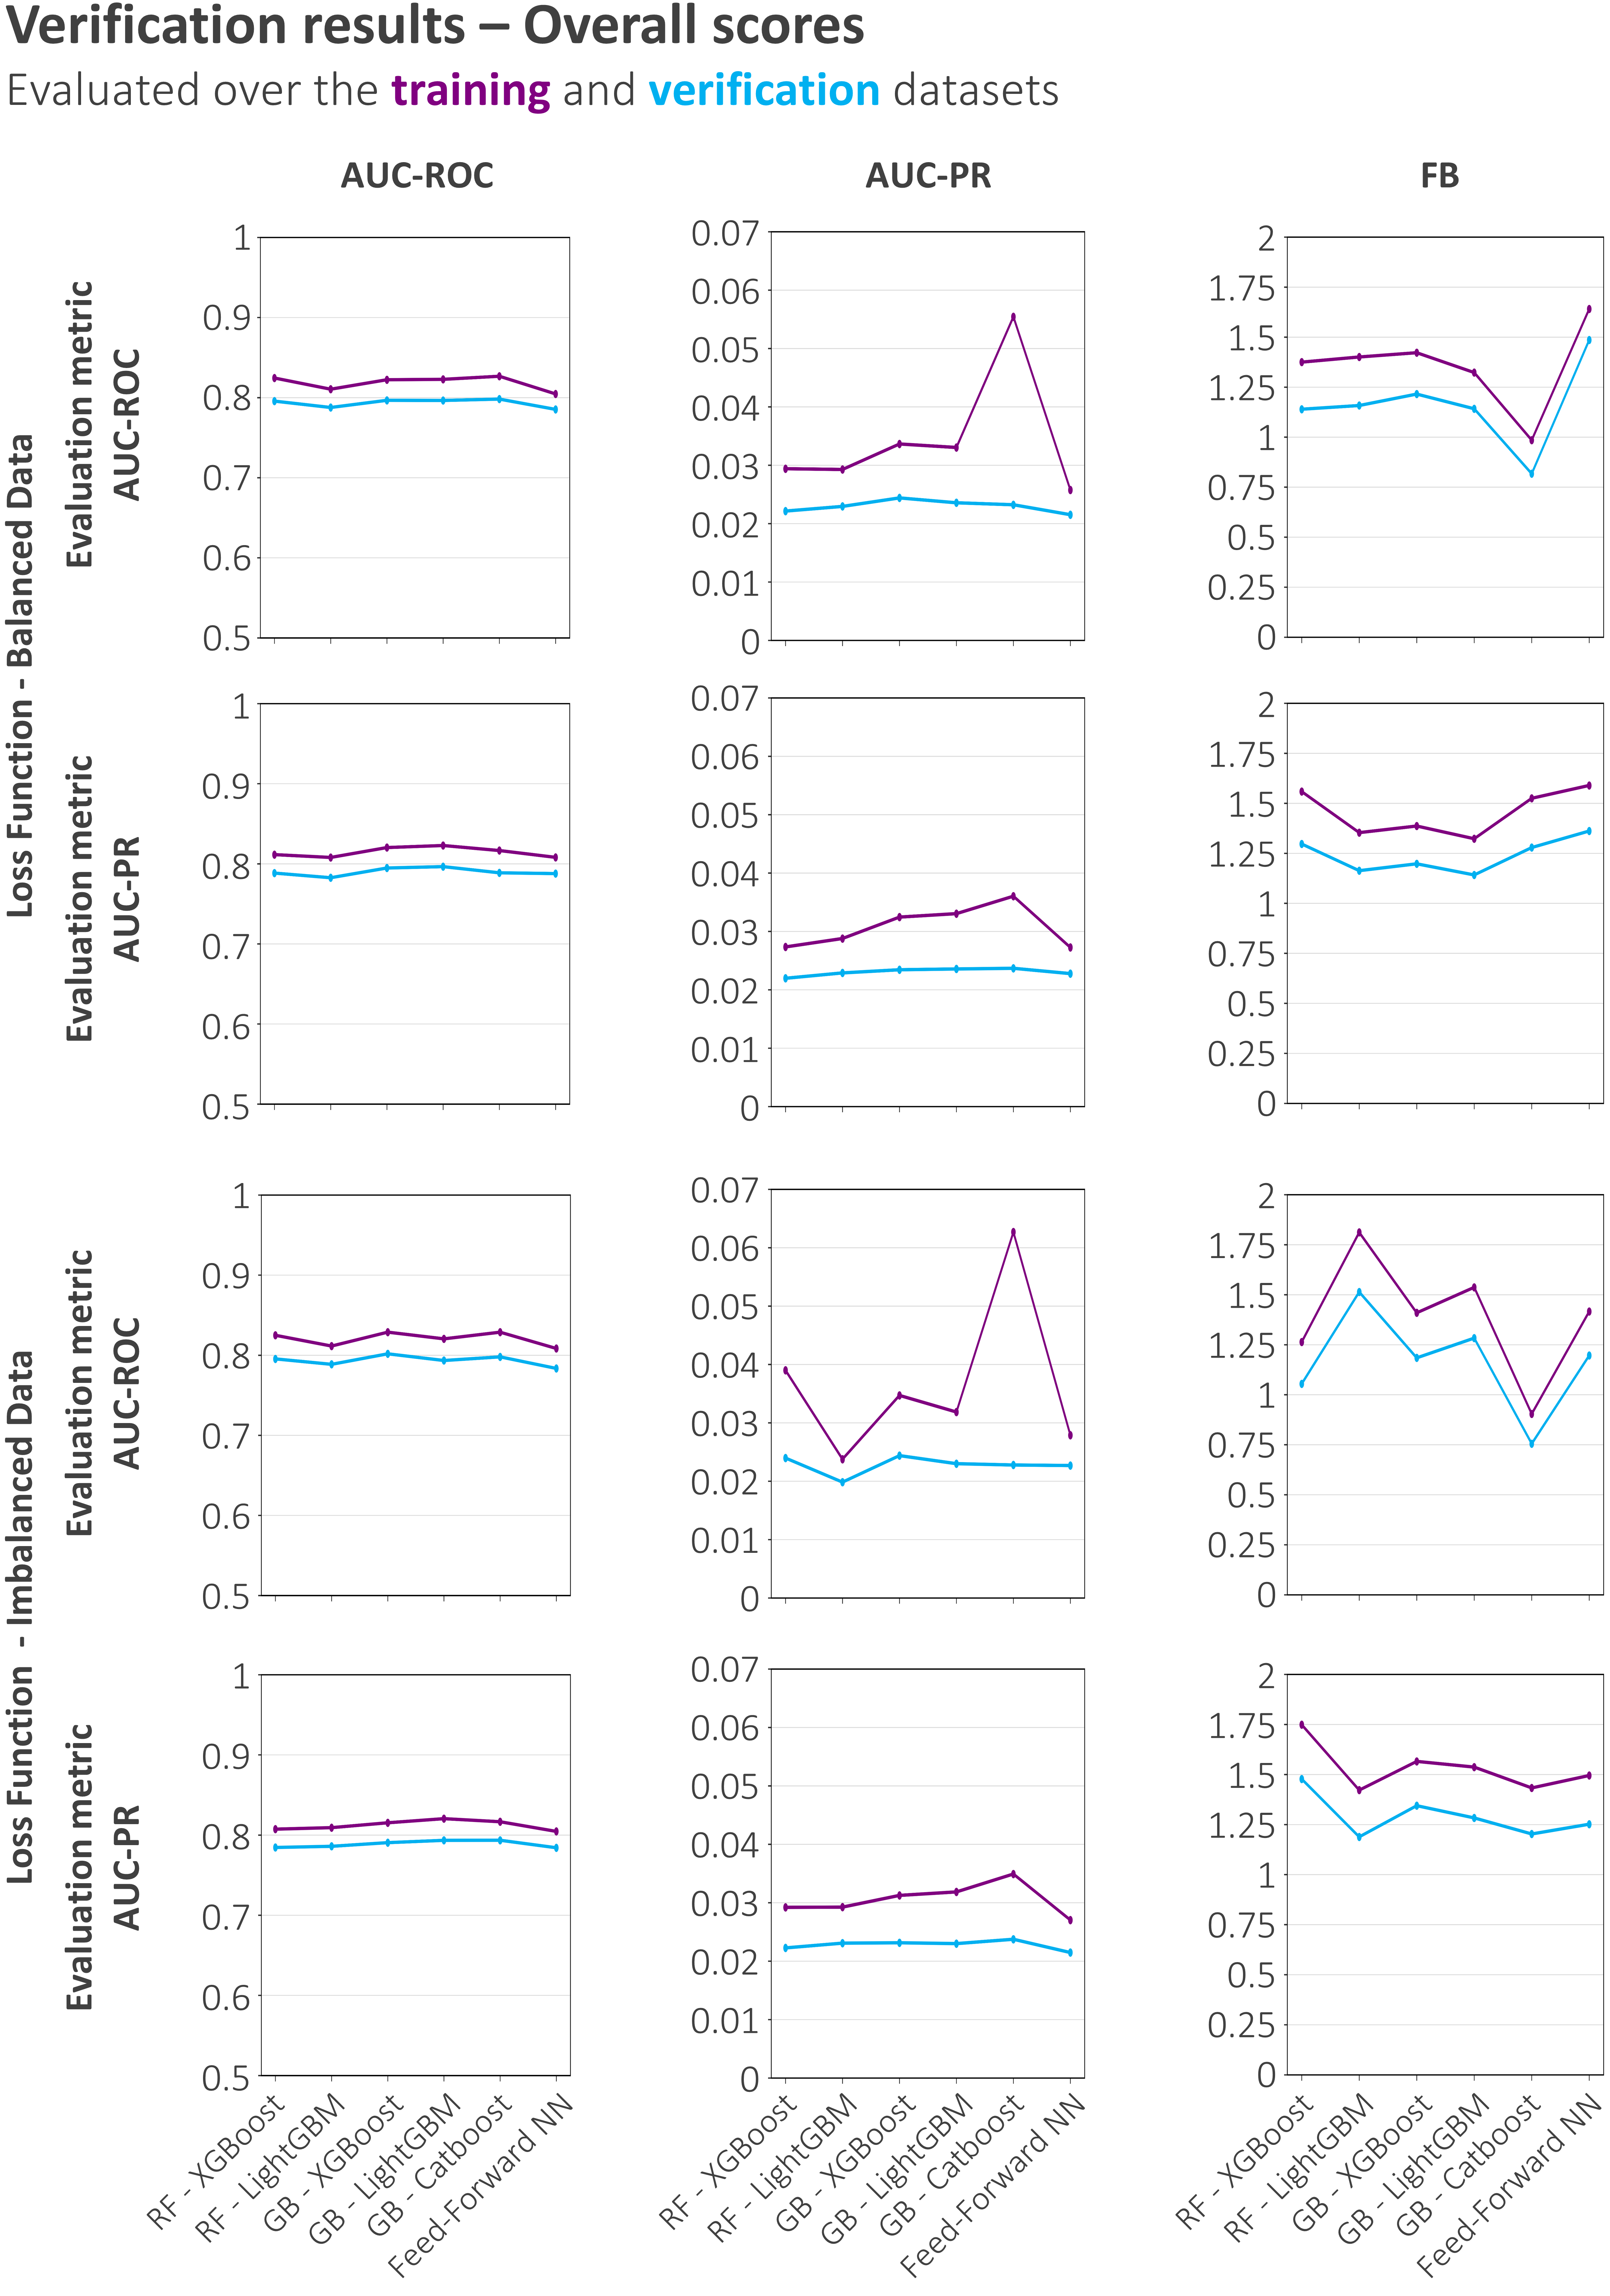
\includegraphics[width=\textwidth]{verif_training_test_overall.png}
\caption{\textbf{Verification results: overall scores} The first, second, and third columns show, respectively, the estimates for the area under the ROC curve (AUC-ROC), the area under the precision-recall curve (AUC-PR), and the frequency bias (FB) for the six considered data-driven models. The estimates of the overall verification scores are shown for the \textcolor{colourTraining}{training dataset} and the \textcolor{colourTest}{verification dataset}. Results are presented for the models trained considering both types of loss functions and evaluation metrics.}
\label{fig:verif_training_test_overall}
\end{figure}

Overall \marginpara{Verification results over reanalysis data: breakdown scores (ROC curves)},
ROC curves exhibit minimal degradation between \textcolor{colourTraining}{training datasets} and \textcolor{colourTest}{verification datasets} (Figure \ref{fig:verif_training_test_breakdown_roc_curve}). The ROC curve, however, reveals distinct patterns between models trained with balanced \ref{fig:verif_training_test_breakdown_roc_curve}a-f and m-r) versus imbalanced loss functions \ref{fig:verif_training_test_breakdown_roc_curve}g-l and s-x). The ROC curves computed for models employing balanced loss functions maintain a remarkably consistent shape across all data-driven models and evaluation metrics, as well as a consistent relative difference between ROC curves computed using the 1\% discretisation (solid lines) and the 0.01\% (dashed lines). The former ROC curves yield lower AUC-ROC values than the latter due to the "truncation effect" caused by stopping the ROC curve at the 1\% probability threshold. The same does not hold when considering models trained with weighted loss functions, except for CatBoost. These ROC curves achieve higher hit rates, e.g., \sim0.9 for the XGBoost and LightGBM implementations of gradient boosting (Figures \ref{fig:verif_training_test_breakdown_roc_curve}i-j) and \sim0.6 for the feed-forward neural network (Figures \ref{fig:verif_training_test_breakdown_roc_curve}l) compared to 0.4 for their balanced counterparts (Figures \ref{fig:verif_training_test_breakdown_roc_curve}c-d and f), but at the cost of much higher false alarm rates, e.g., \sim0.5 for XGBoost and LightGBM an \sim0.2 for the feed-forward neural network compared to 0.025 in their balanced counterparts. Whilst XGBoost and LightGBM implementations of gradient boosting and the feed-forward neural network show consistent patterns across evaluation metrics, the random forest implementations display metric-dependent responses. Specifically, LightGBM Random Forest shows the altered behaviour when optimised for AUC-ROC, whereas XGBoost Random Forest responds differently under AUC-PR.

\begin{figure}[htbp]
\centering
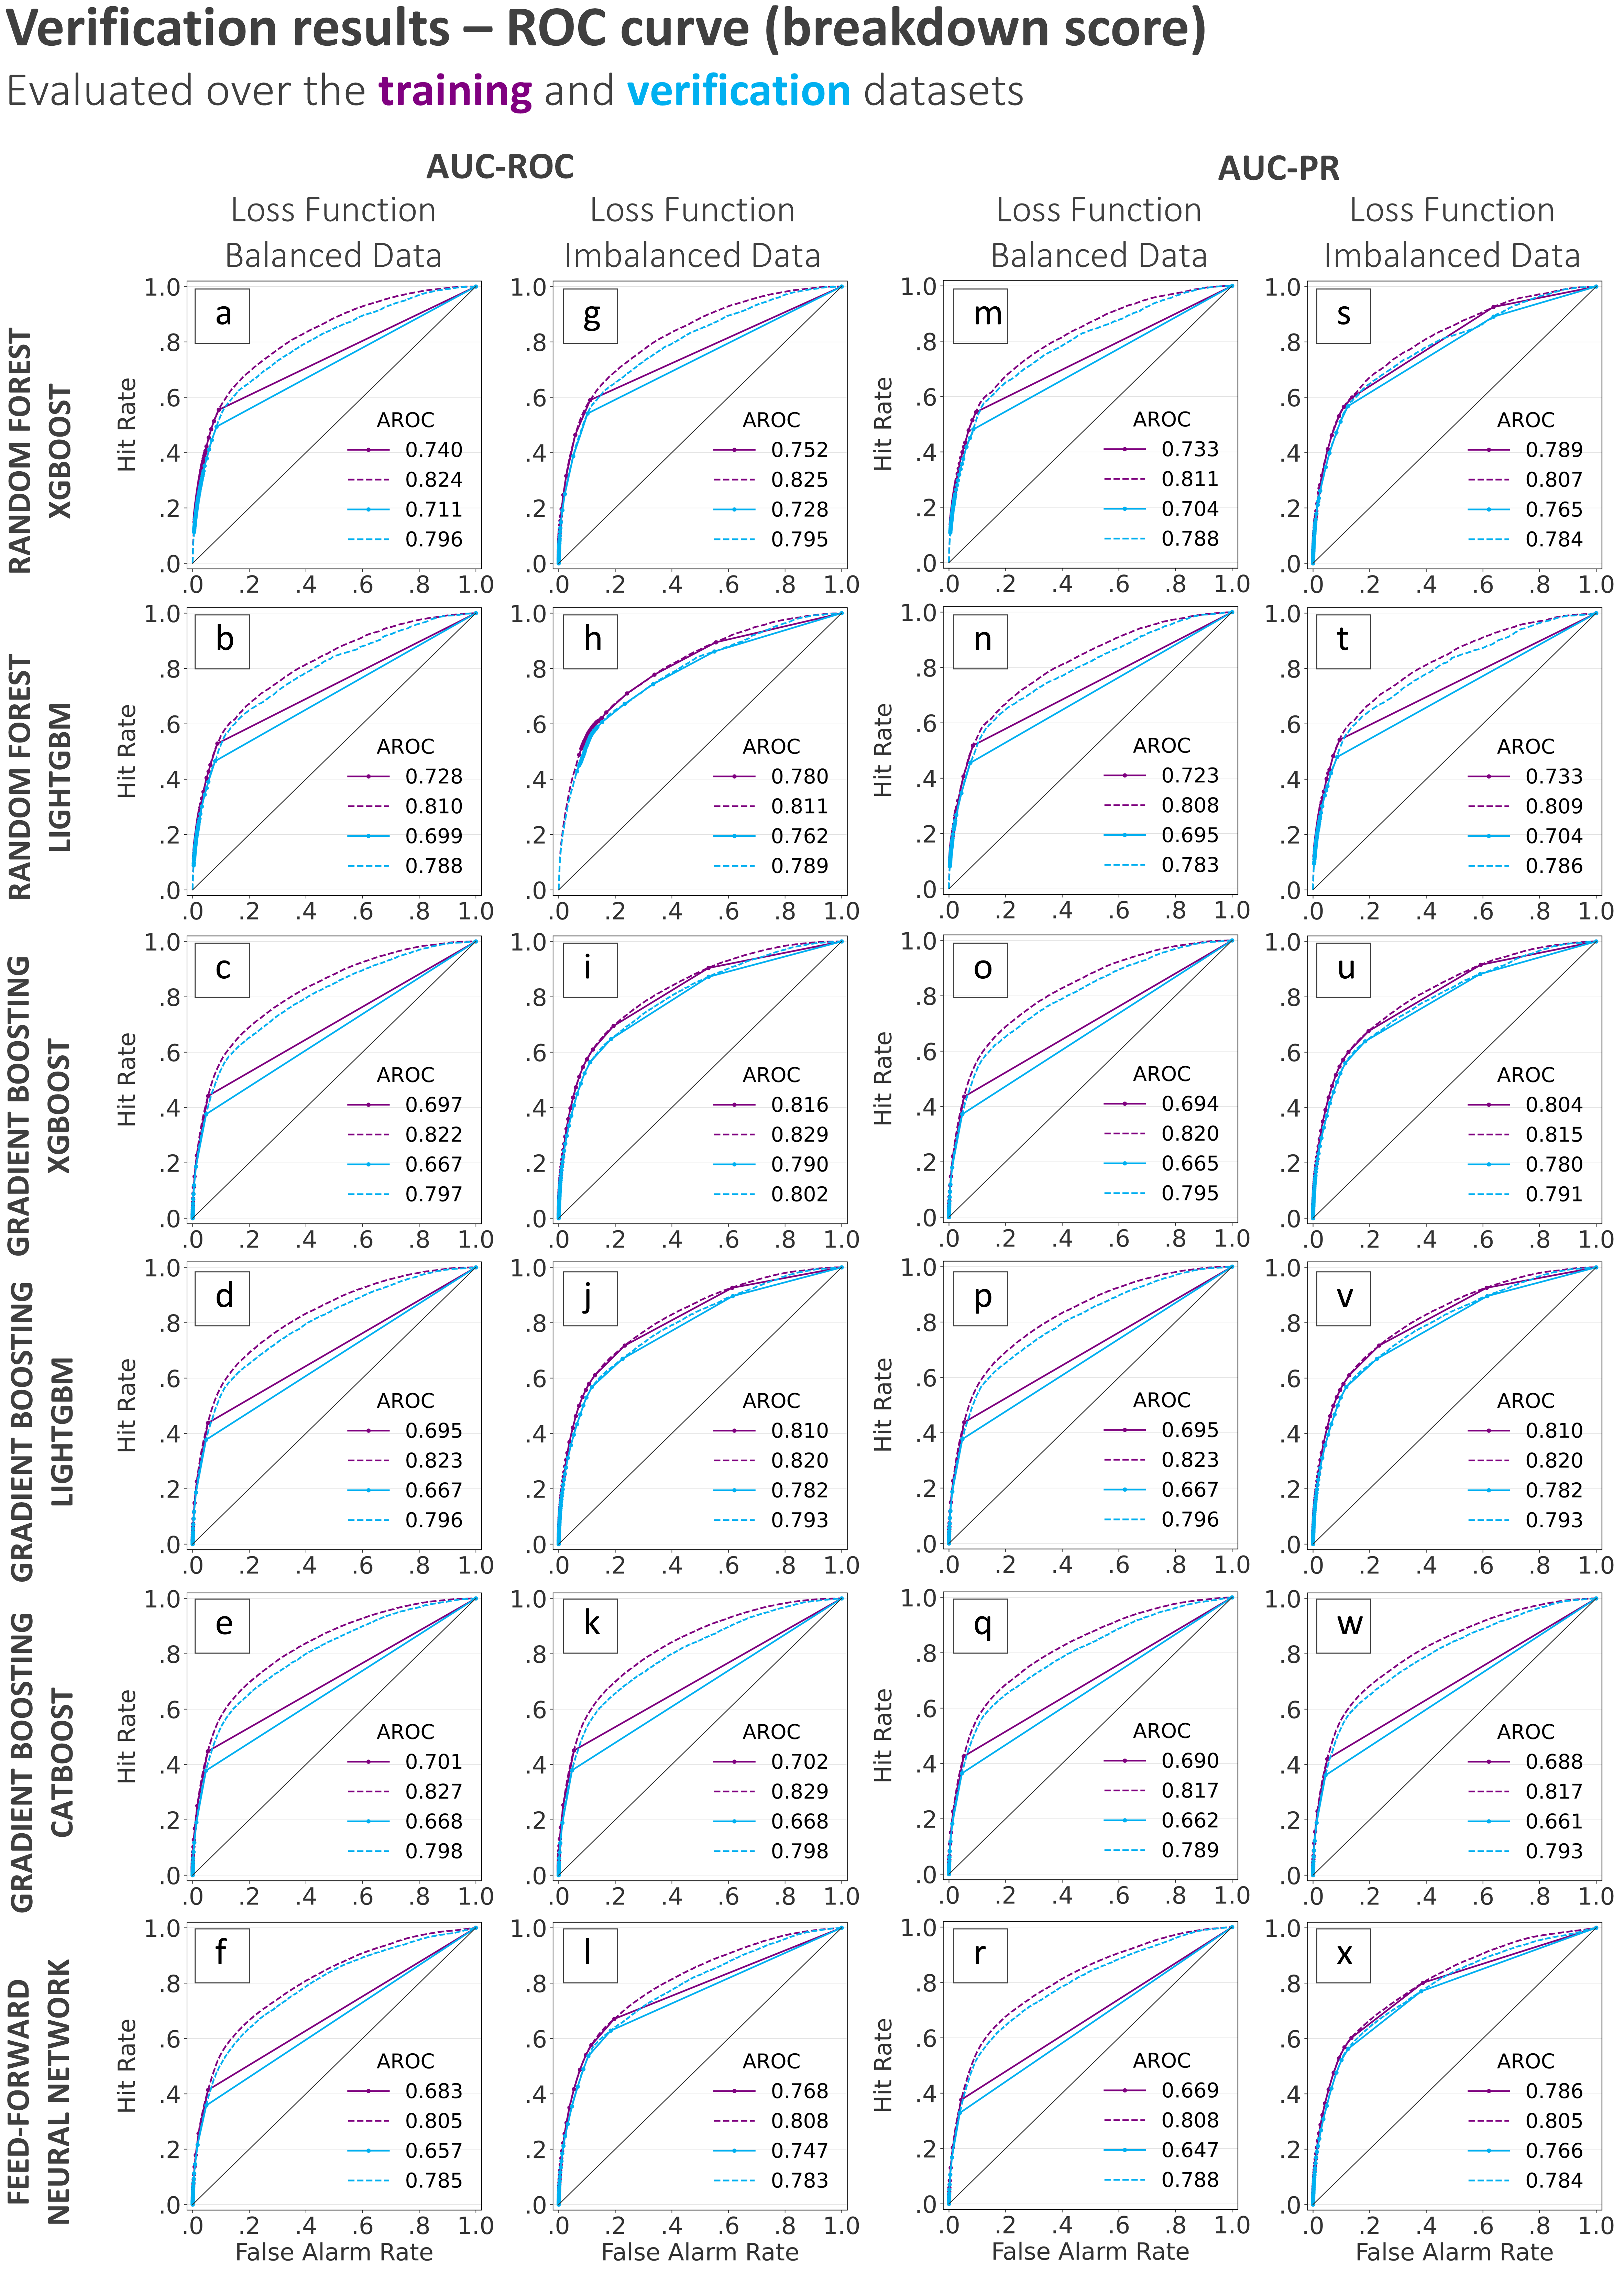
\includegraphics[width=\textwidth]{verif_training_test_breakdown_roc_curve.png}
\caption{\textbf{Verification results: breakdown scores (ROC curves)} ROC curves computed for the \textcolor{colourTraining}{training dataset} and the \textcolor{colourTest}{verification dataset}, for six data-driven models (from top to bottom): random forest XGBoost, random forest LightGBM, gradient boosting XGBoost, gradient boosting LightGBM, gradient boosting CatBoost, and feed-forward neural network. The solid lines represent ROC curves computed considering forecast probabilities discretised every 1\%, whilst the dashed lines represent ROC curves computed using a finer discretisation of probabilities (0.01\%). ROC curves are shown for the two evaluation metrics (AUC-ROC - panels (a) to (l) - and AUC-PR - panels (m) to (x)) and types of loss function configurations (balanced and imbalanced datasets) considered during the training of the data-driven models.}
\label{fig:verif_training_test_breakdown_roc_curve}
\end{figure}

Overall \marginpara{Verification results over reanalysis data: breakdown scores (Precision-Recall curves)}, the precision-recall curves exhibit minimal degradation between \textcolor{colourTraining}{training datasets} (in solid lines) and \textcolor{colourTest}{verification datasets} (in dashed lines), with the major differences concentrated mainly over recall values smaller than 0.2 (Figure \ref{fig:verif_training_test_breakdown_pr_curve}). All precision-recall curves, while obtaining fairly small values of AUC-PR (see Figure \ref{fig:verif_training_test_overall}, second column), remain away from their corresponding lines of no skill (grey solid lines for the training dataset and grey dashed line for the test dataset, which mostly overlap). Whilst there are some differences between the precision-recall curves attributable to the differences in model training, this time (as opposed to what was seen for the ROC curves), the most considerable differences are observed between the models themselves. In all implementations of gradient boosting (Figures \ref{fig:verif_training_test_breakdown_pr_curve}c-e, i-k, o-q, and u-v), the \textcolor{colourTraining}{training datasets} achieve high precision (between 0.6 and 1) over very small values of recall, while the \textcolor{colourTest}{verification datasets} achieve a precision value between 0.2 and 0.6. Only CatBoost, trained with the weighted loss function, maintains the value of 1. In the feed-forward neural network (\ref{fig:verif_training_test_breakdown_pr_curve}f, l, r, and x), the precision-recall curve remains virtually identical between the \textcolor{colourTraining}{training datasets} and the \textcolor{colourTest}{verification datasets}, including at very low values of recall. Finally, both XGBoost and LightGBM implementations of random forest show very different precision-recall curves. LightGBM (\ref{fig:verif_training_test_breakdown_pr_curve}b, h, n, and t) shows a precision-recall curve that begins at recall values between 0.2 and 0.4, and precision values that do not exceed 0.1. XGBoost shows a similar behaviour when the model is trained using the generic loss function (\ref{fig:verif_training_test_breakdown_pr_curve}a and m), whilst the curves for the models trained with the weighted loss function (\ref{fig:verif_training_test_breakdown_pr_curve}g and s) shows a shape that is similar to that for the corresponding XGBoost implementation of gradient boosting (\ref{fig:verif_training_test_breakdown_pr_curve}i and u).

\begin{figure}[htbp]
\centering
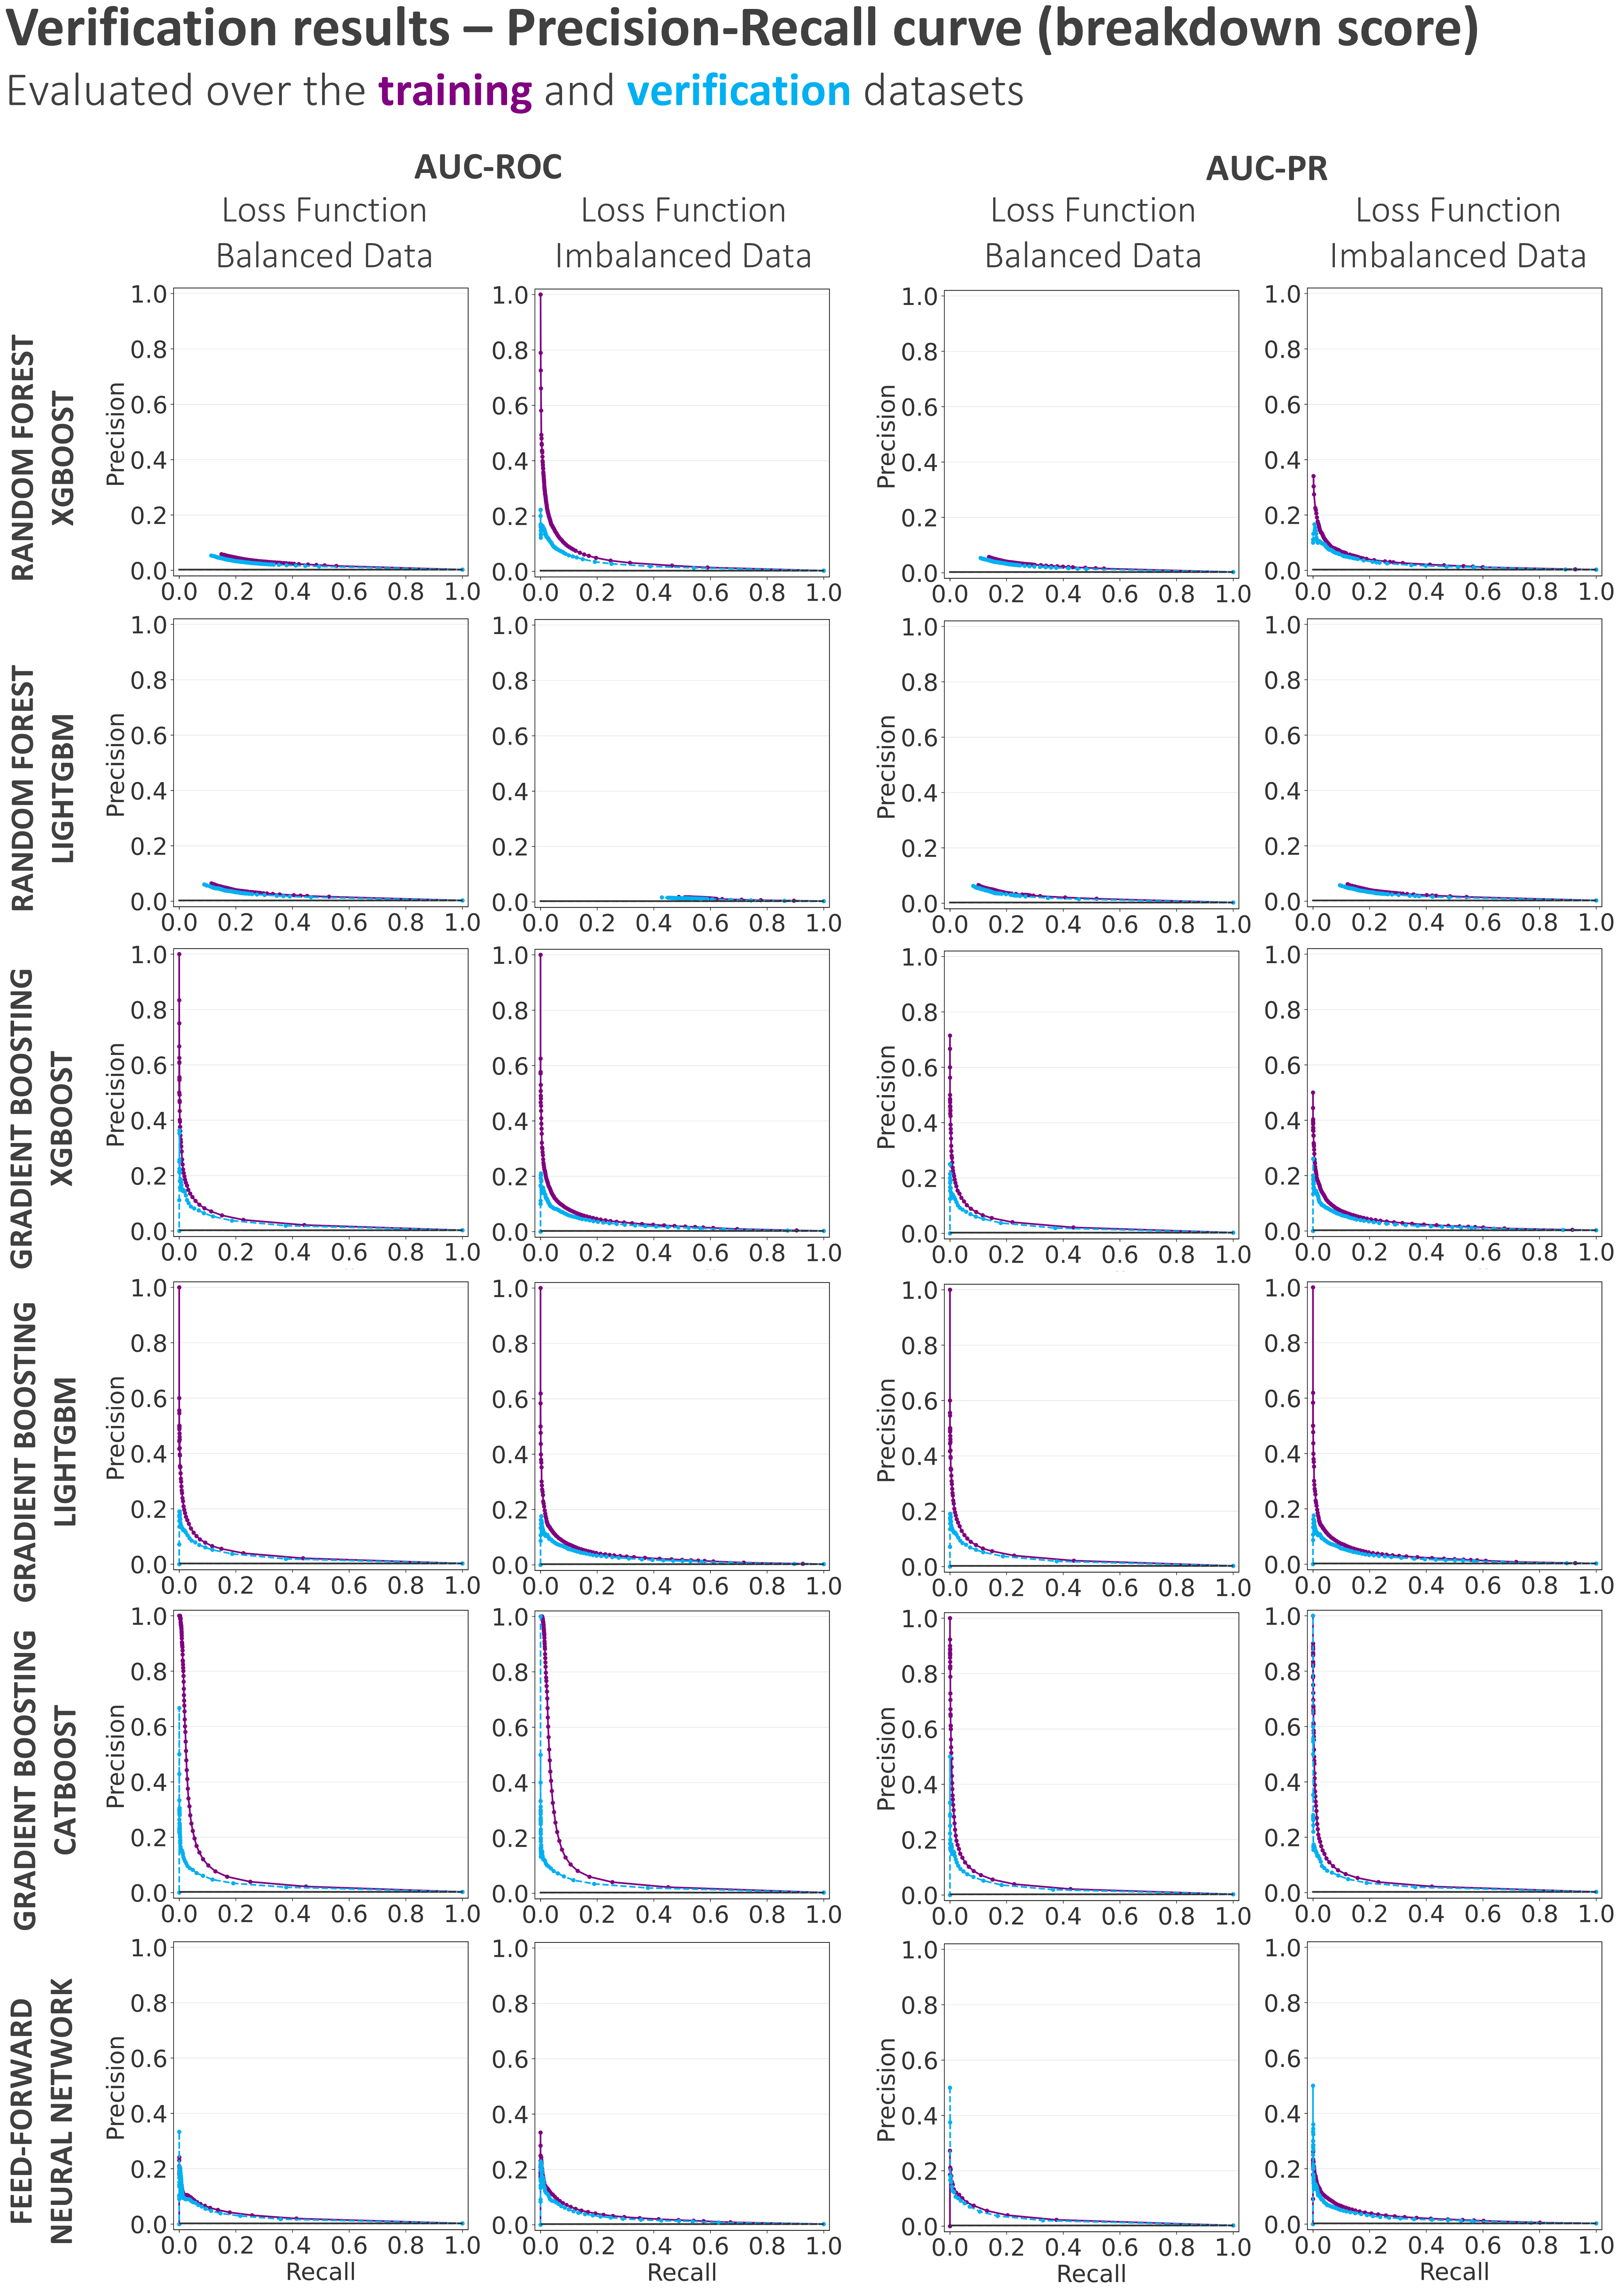
\includegraphics[width=\textwidth]{verif_training_test_breakdown_pr_curve.png}
\caption{\textbf{Verification results: breakdown scores (Precision-Recall curves)} Similar to Figure \ref{fig:verif_training_test_breakdown_roc_curve} but for the Precision-Recall curve} 
\label{fig:verif_training_test_breakdown_pr_curve}
\end{figure}

Overall \marginpara{Verification results over reanalysis data: breakdown scores (Reliability diagrams)}, the reliability diagrams exhibit minimal degradation between \textcolor{colourTraining}{training datasets} and \textcolor{colourTest}{verification datasets}, but it increases with increasing forecast probabilities (Figure \ref{fig:verif_training_test_breakdown_reliability_diagram}). Models trained with balanced loss functions (Figures \ref{fig:verif_training_test_breakdown_reliability_diagram}a-f and m-r) demonstrate different calibration characteristics compared to those using weighted loss functions \ref{fig:verif_training_test_breakdown_reliability_diagram}g-l and s-x). For models trained with balanced loss functions, the gradient boosting implementations and the feed-forward neural network yield reliable forecast probabilities under 10\% (20\% for XGBoost). At higher probability ranges, where predictions become less frequent and diagrams noisier, distinct patterns emerge. LightGBM and XGBoost show mostly reliable probabilities across all probability ranges (Figures \ref{fig:verif_training_test_breakdown_reliability_diagram}c-d and o-p). CatBoost systematically underestimates forecast probabilities (Figures \ref{fig:verif_training_test_breakdown_reliability_diagram}e and q). The feed-forward neural network shows contrasting behaviour depending on the evaluation metric used during hyperparameter tuning: overestimation occurs when tuned for AUC-ROC (Figure \ref{fig:verif_training_test_breakdown_reliability_diagram}f), while forecast probabilities remain reliable when tuned considering AUC-PR (Figure \ref{fig:verif_training_test_breakdown_reliability_diagram}r). Models trained with weighted loss functions (Figures \ref{fig:verif_training_test_breakdown_reliability_diagram}g-l and s-x) display systematic overestimation across the entire probability spectrum, except for CatBoost, which maintains similar calibration patterns to its balanced function counterpart. Random forest implementations show systematic overestimations independent of the considered loss function \ref{fig:verif_training_test_breakdown_reliability_diagram}a-b, g-h, m-n, and s-t).

\begin{figure}[htbp]
\centering
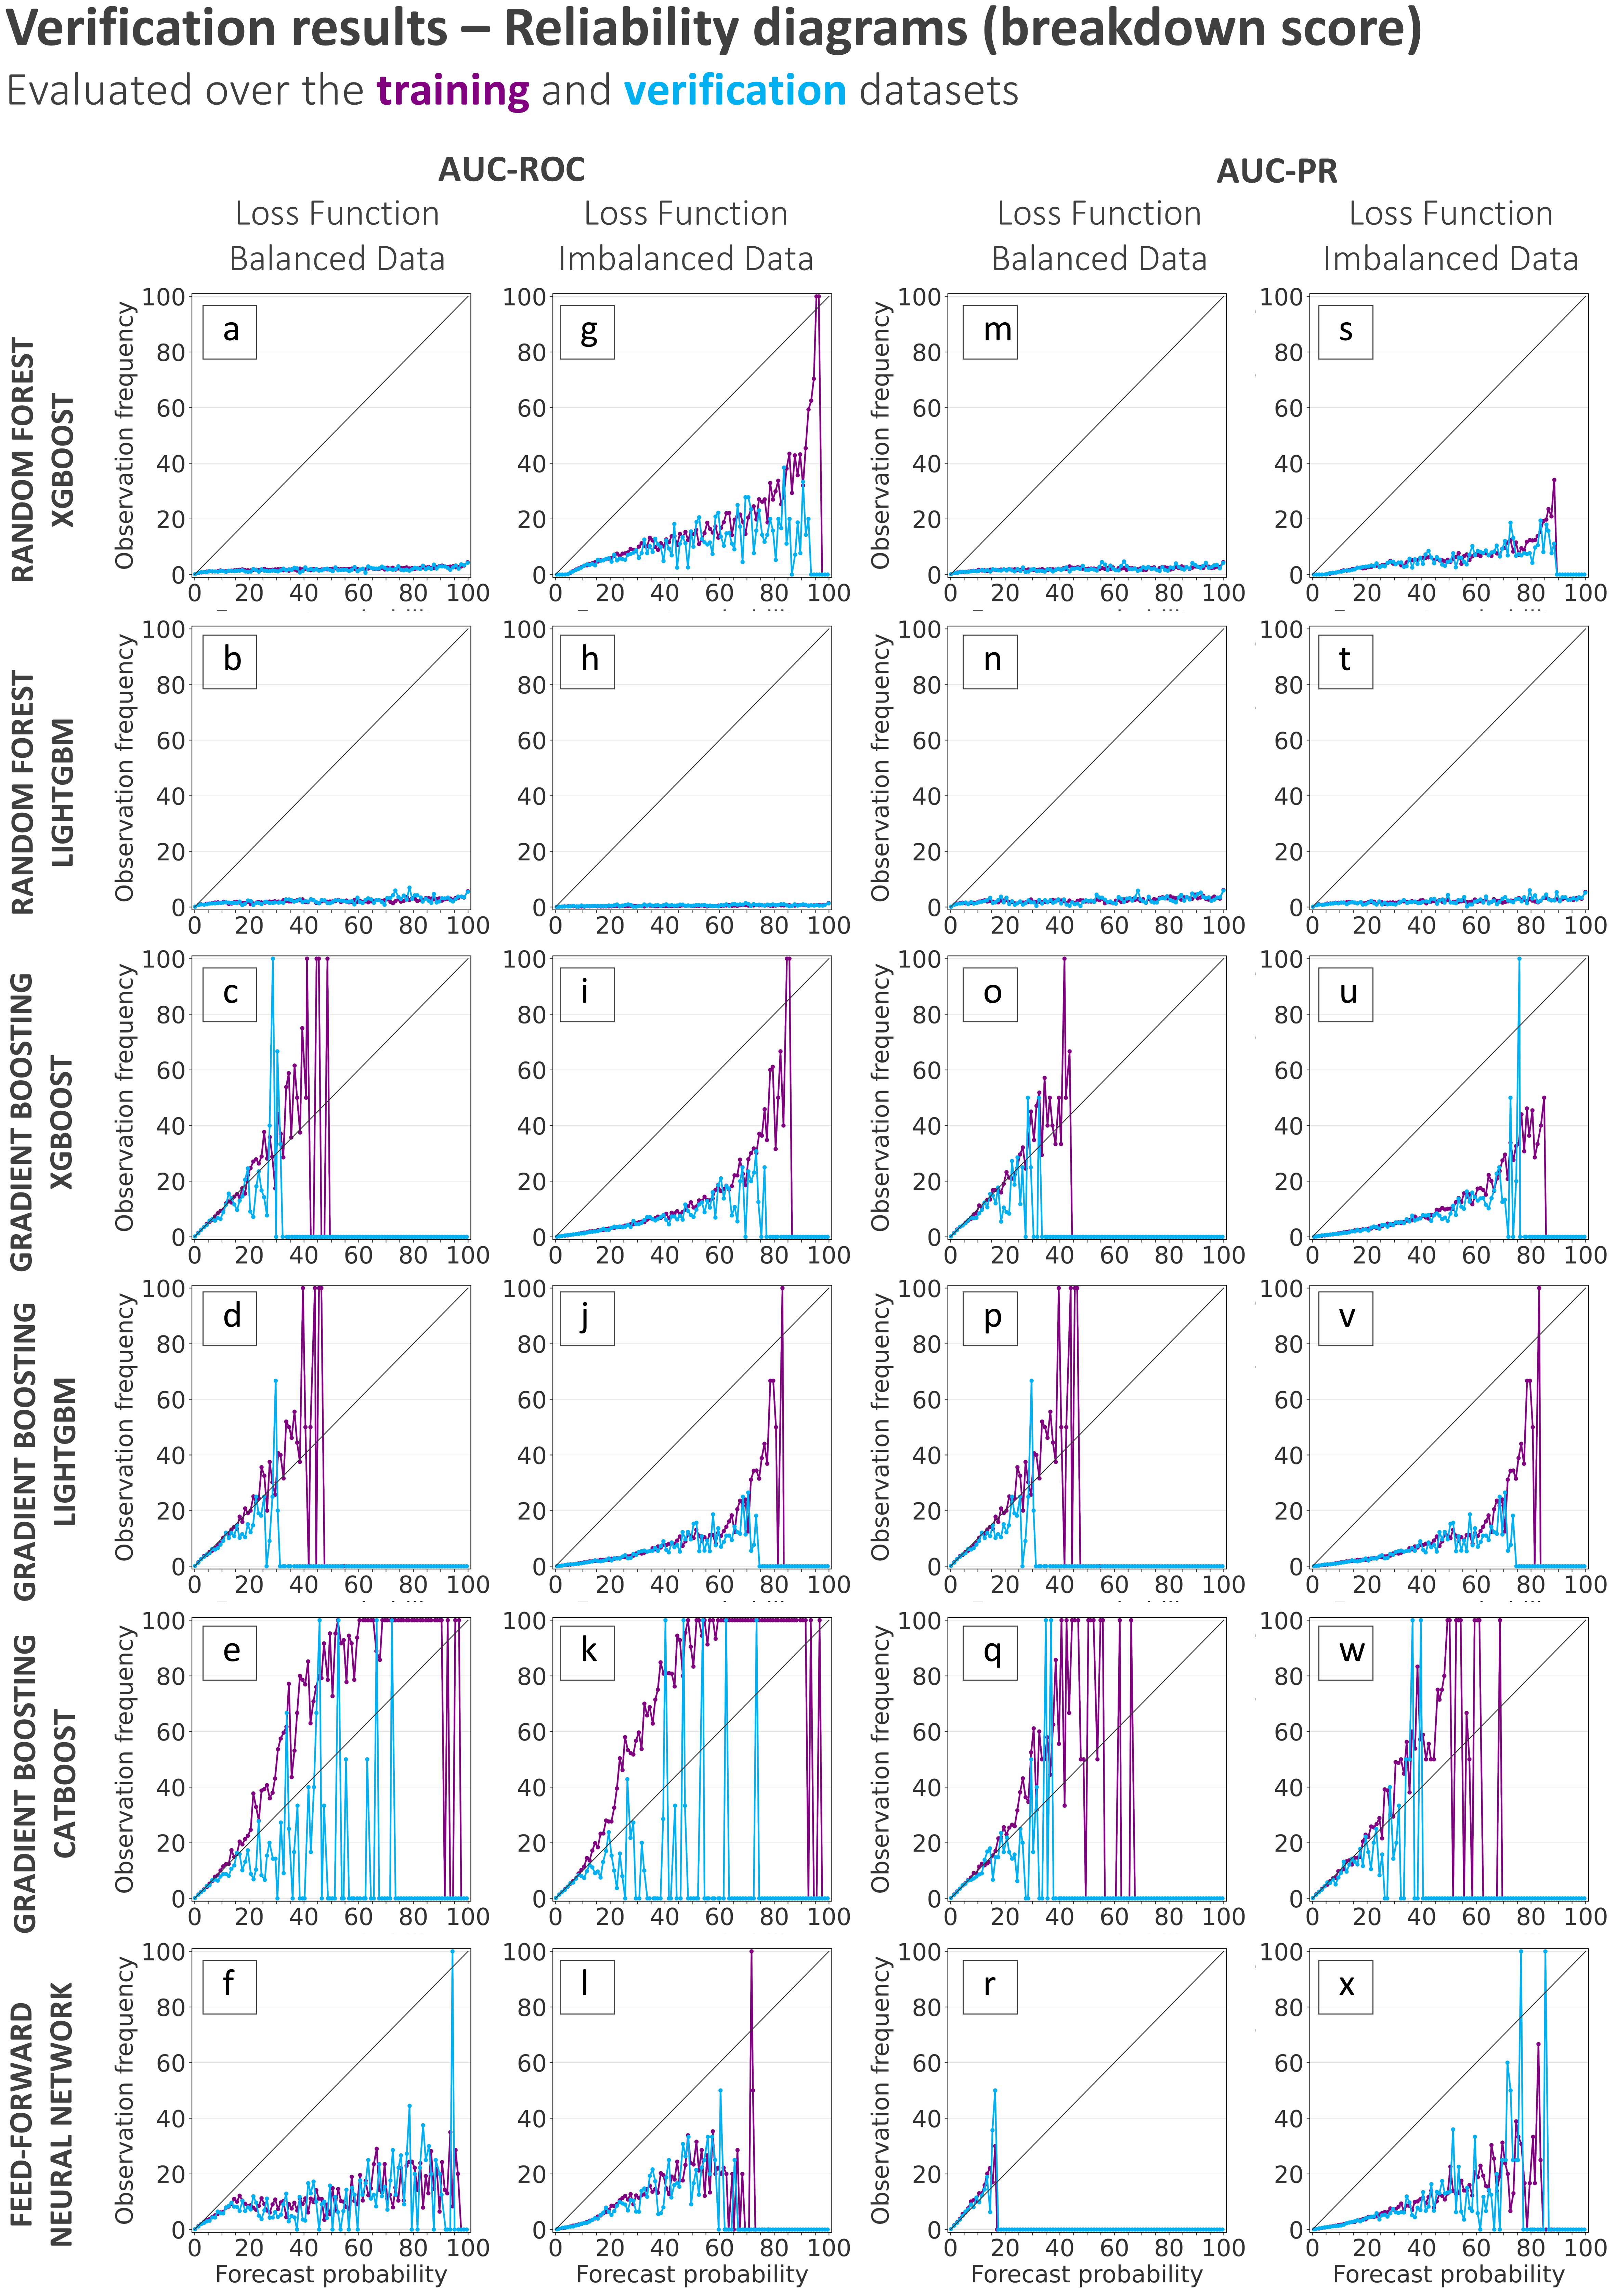
\includegraphics[width=\textwidth]{verif_training_test_breakdown_reliability_diagram.png}
\caption{\textbf{Verification results: breakdown scores (Reliability diagrams)} Similar to Figure \ref{fig:verif_training_test_breakdown_roc_curve} but for reliability diagrams.}
\label{fig:verif_training_test_breakdown_reliability_diagram}
\end{figure}


\subsection{Verification results over forecast data}

\begin{figure}[htbp]
\centering
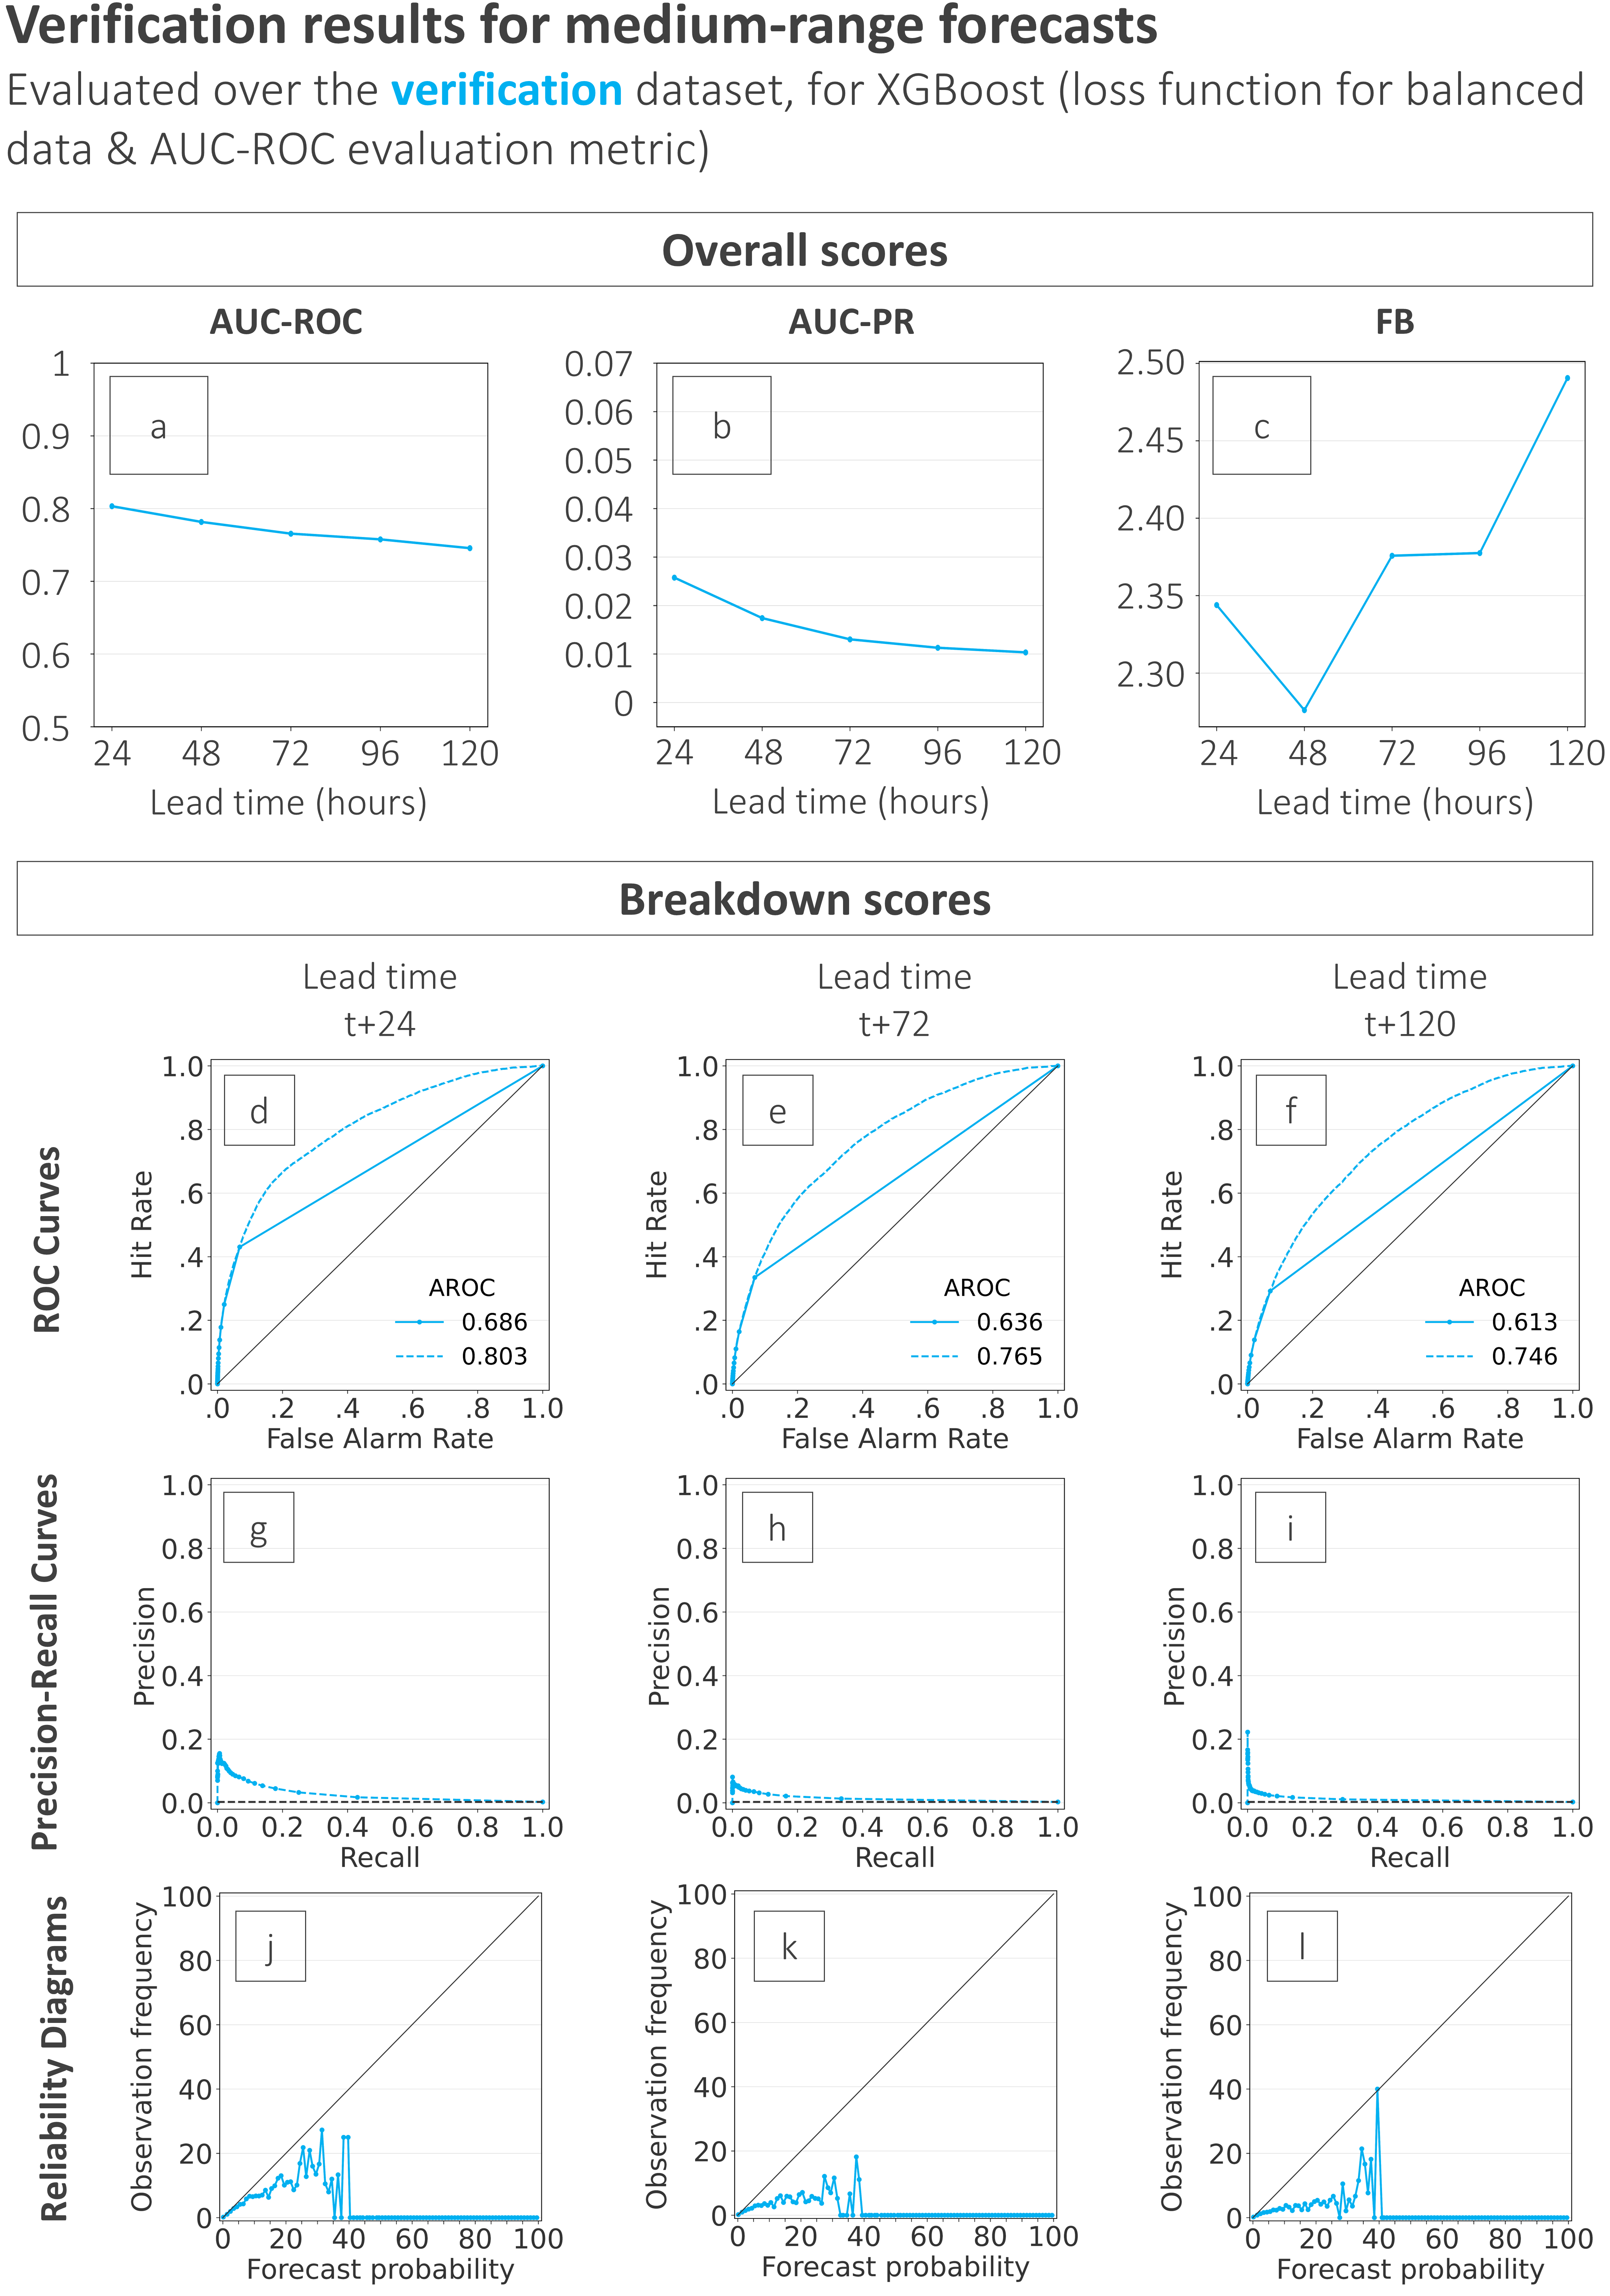
\includegraphics[width=\textwidth]{chapter_06/figures/verif_long_fc.png}
\caption{\textbf{Verification results for medium-range forecasts for XGBoost implementation of gradient boosting (trained with the loss function for balanced data and hyperparameters maximised for AUC-ROC).} Panels (a) to (c) show the overall scores, respectively, for the area under the ROC curve (AUC-ROC), the area under the precision-recall curve (AUC-PR), and the frequency bias (FB). The remaining panels show the breakdown scores, respectively, for the ROC curves (Panels (d) to (f)), the Precision-Recall curves (Panels (g) to (i)), and for the Reliability Diagram (Panels (j) to (l)).}
\label{fig:verif_long_fc}
\end{figure}





%%%%%%%%%%%%%%%%%%%%%%%%%%%%%%%%%%%%%%%%%%%%%%%%%%%%%%%%%%%%%%%%%%%%%%%
\section{Physical interpretation of the data-driven model behaviour}
\label{data_driven_flash_floods_short_medium_range_physical_interpretation}

For the sake of brevity and clarity, the following section will present SHAP-related plots exclusively for the XGBoost implementation of gradient boosting, trained with the balanced loss function and optimised for AUC-ROC. This representative configuration was selected because the feature importance patterns and SHAP value distributions demonstrate remarkable consistency across all model architectures, loss function configurations, and evaluation metrics examined in this study. 


Preliminary analysis confirmed that the relative importance rankings and interaction patterns remain substantially unchanged regardless of the specific implementation, thus rendering exhaustive presentation of all permutations redundant without providing additional analytical insights. The selected configuration serves as an exemplar that effectively captures the universal patterns observed across the entire model ensemble, allowing for a focused discussion of the hydro-meteorological drivers of flash flood risk without unnecessary repetition.









%%%%%%%%%%%%%%%%%%%%%
\section{Discussions}
\label{data_driven_flash_floods_short_medium_range_discussions}
% Still to be completed.


%%%%%%%%%%%%%%%%%%%%%
\section{Conclusions}
\label{data_driven_flash_floods_short_medium_range_conclusions}
% Still to be completed.